
%  A simple AAU report template.
%  2015-05-08 v. 1.2.0
%  Copyright 2010-2015 by Jesper Kjær Nielsen <jkn@es.aau.dk>
%
%  This is free software: you can redistribute it and/or modify
%  it under the terms of the GNU General Public License as published by
%  the Free Software Foundation, either version 3 of the License, or
%  (at your option) any later version.
%
%  This is distributed in the hope that it will be useful,
%  but WITHOUT ANY WARRANTY; without even the implied warranty of
%  MERCHANTABILITY or FITNESS FOR A PARTICULAR PURPOSE.  See the
%  GNU General Public License for more details.
%
%  You can find the GNU General Public License at <http://www.gnu.org/licenses/>.
%
\documentclass[11pt,a4paper,openright,openany]{report}
%\documentclass[xcolor=table]{beamer}
\usepackage[hidelinks]{hyperref}
\usepackage[toc,page]{appendix}
\usepackage{wrapfig}
\usepackage{listings}
\usepackage{color}
\usepackage{subcaption}
\usepackage{textcomp}
\usepackage{pdfpages}
\usepackage{gensymb}
%\usepackage[parfill]{parskip}
\usepackage{blindtext}
\usepackage{float}
\setcounter{secnumdepth}{3}
\setcounter{tocdepth}{2}
\usepackage[table,xcdraw]{xcolor}
\providecommand{\tightlist}{%
  \setlength{\itemsep}{0pt}\setlength{\parskip}{0pt}}
%%%%%%%%%%%%%%%%%%%%%%%%%%%%%%%%%%%%%%%%%%%%%%%%
% Language, Encoding and Fonts
% http://en.wikibooks.org/wiki/LaTeX/Internationalization
%%%%%%%%%%%%%%%%%%%%%%%%%%%%%%%%%%%%%%%%%%%%%%%%
% Select encoding of your inputs. Depends on
% your operating system and its default input
% encoding. Typically, you should use
%   Linux  : utf8 (most modern Linux distributions)
%            latin1
%   Windows: ansinew
%            latin1 (works in most cases)
%   Mac    : applemac
% Notice that you can manually change the input
% encoding of your files by selecting "save as"
% an select the desired input encoding.
\usepackage[utf8]{inputenc}
% Make latex understand and use the typographic
% rules of the language used in the document.
\usepackage[danish,english]{babel}
%\usepackage[danish]{babel}
% Use the palatino font
\usepackage[sc]{mathpazo}
\linespread{1.05}         % Palatino needs more leading (space between lines)
% Choose the font encoding
\usepackage[T1]{fontenc}
%%%%%%%%%%%%%%%%%%%%%%%%%%%%%%%%%%%%%%%%%%%%%%%%
% Graphics and Tables
% http://en.wikibooks.org/wiki/LaTeX/Importing_Graphics
% http://en.wikibooks.org/wiki/LaTeX/Tables
% http://en.wikibooks.org/wiki/LaTeX/Colors
%%%%%%%%%%%%%%%%%%%%%%%%%%%%%%%%%%%%%%%%%%%%%%%%
% load a colour package
\usepackage{xcolor}
\definecolor{aaublue}{RGB}{33,26,82}% dark blue
\definecolor{color5}{RGB}{10,56,74}
\definecolor{color4}{RGB}{2,66,83}
\definecolor{color3}{RGB}{96,150,145}
\definecolor{color2}{RGB}{194,210,196}
\definecolor{color1}{RGB}{233,243,244}
% The standard graphics inclusion package
\usepackage{graphicx}

%More languages
\usepackage{inc/listings-golang}
\usepackage{inc/json}
\usepackage{inc/docker}
\renewcommand{\lstlistingname}{Code-block}
\renewcommand{\lstlistlistingname}{List of \lstlistingname s}
% Set up how figure and table captions are displayed
\usepackage{caption}
\captionsetup{%
  font=footnotesize,% set font size to footnotesize
  labelfont=bf % bold label (e.g., Figure 3.2) font
}
% Make the standard latex tables look so much better
\usepackage{array,booktabs}
% Enable the use of frames around, e.g., theorems
% The framed package is used in the example environment
\usepackage{framed}
\definecolor{graphblue}{HTML}{437EAA}
\definecolor{listinggray}{HTML}{E8F5FD}
\lstset{
	backgroundcolor=\color{color1},
	tabsize=4,
	language=Golang,
    language=JSON,
    language=docker,
    language=docker-compose,
	rulecolor=,
	language=matlab,
        basicstyle=\scriptsize,
        upquote=true,
        captionpos=b,
        aboveskip={1.5\baselineskip},
        columns=fixed,
        showstringspaces=false,
        extendedchars=true,
        breaklines=true,
        prebreak = \raisebox{0ex}[0ex][0ex]{\ensuremath{\hookleftarrow}},
        frame=single,
        showtabs=false,
        showspaces=false,
        showstringspaces=false,
        identifierstyle=\ttfamily,
        keywordstyle=\color[rgb]{0,0,1},
        commentstyle=\color[rgb]{0.133,0.545,0.133},
        stringstyle=\color[rgb]{0.627,0.126,0.941},
}

%%%%%%%%%%%%%%%%%%%%%%%%%%%%%%%%%%%%%%%%%%%%%%%%
% Mathematics
% http://en.wikibooks.org/wiki/LaTeX/Mathematics
%%%%%%%%%%%%%%%%%%%%%%%%%%%%%%%%%%%%%%%%%%%%%%%%
% Defines new environments such as equation,
% align and split
\usepackage{amsmath}
% Adds new math symbols
\usepackage{amssymb}
% Use theorems in your document
% The ntheorem package is also used for the example environment
% When using thmmarks, amsmath must be an option as well. Otherwise \eqref doesn't work anymore.
\usepackage[framed,amsmath,thmmarks]{ntheorem}
\usepackage[toc]{glossaries}
% cleverref
\usepackage[capitalise,noabbrev]{cleveref}
\crefname{listing}{Code-block}{Code-block}
\Crefname{listing}{Code-block}{Code-block}
\crefname{appsec}{Appendix}{Appendices}
\crefname{appsubsec}{Appendix}{Appendices}

%%%%%%%%%%%%%%%%%%%%%%%%%%%%%%%%%%%%%%%%%%%%%%%%
% Page Layout
% http://en.wikibooks.org/wiki/LaTeX/Page_Layout
%%%%%%%%%%%%%%%%%%%%%%%%%%%%%%%%%%%%%%%%%%%%%%%%
% Change margins, papersize, etc of the document
\usepackage[
  inner=28mm,% left margin on an odd page
  outer=41mm,% right margin on an odd page
  ]{geometry}
% Modify how \chapter, \section, etc. look
% The titlesec package is very configureable
\usepackage{titlesec}
%\titleformat{\chapter}[display]{\normalfont\huge\bfseries}{\chaptertitlename\ \thechapter}{20pt}{\Huge}
\titleformat{\chapter}{\normalfont\huge}{\thechapter}{20pt}{\Huge}
\titleformat*{\section}{\normalfont\Large\bfseries}
\titleformat*{\subsection}{\normalfont\large\bfseries}
\titleformat*{\subsubsection}{\normalfont\normalsize\bfseries}
%\titleformat*{\paragraph}{\normalfont\normalsize\bfseries}
%\titleformat*{\subparagraph}{\normalfont\normalsize\bfseries}
\titlespacing*{\chapter}{0pt}{0pt}{40pt}
%https://tex.stackexchange.com/questions/299969/titlesec-loss-of-section-numbering-with-the-new-update-2016-03-15

% Clear empty pages between chapters
\let\origdoublepage\cleardoublepage
\newcommand{\clearemptydoublepage}{%
  \clearpage
  {\pagestyle{empty}\origdoublepage}%
}
\let\cleardoublepage\clearemptydoublepage

% Change the headers and footers
\usepackage{fancyhdr}
\pagestyle{fancy}
\fancyhf{} %delete everything
\renewcommand{\headrulewidth}{0pt} %remove the horizontal line in the header
\fancyhead[RE]{\small\nouppercase\leftmark} %even page - chapter title
\fancyhead[LO]{\small\nouppercase\rightmark} %uneven page - section title
\fancyhead[LE,RO]{\thepage} %page number on all pages
% Do not stretch the content of a page. Instead,
% insert white space at the bottom of the page
\raggedbottom
% Enable arithmetics with length. Useful when
% typesetting the layout.
\usepackage{calc}

%%%%%%%%%%%%%%%%%%%%%%%%%%%%%%%%%%%%%%%%%%%%%%%%
% Bibliography
% http://en.wikibooks.org/wiki/LaTeX/Bibliography_Management
%%%%%%%%%%%%%%%%%%%%%%%%%%%%%%%%%%%%%%%%%%%%%%%%
\usepackage[backend=bibtex,
  bibencoding=utf8
  ]{biblatex}
\addbibresource{bib/mybib}

%%%%%%%%%%%%%%%%%%%%%%%%%%%%%%%%%%%%%%%%%%%%%%%%
%%%%%%%%%%%%%%%%%%%%%%%%%%%%%%%%%%%%%%%%%%%%%%%%
% Misc
%%%%%%%%%%%%%%%%%%%%%%%%%%%%%%%%%%%%%%%%%%%%%%%%
% Add bibliography and index to the table of
% contents
\usepackage[nottoc]{tocbibind}
% Add the command \pageref{LastPage} which refers to the
% page number of the last page
\usepackage{lastpage}
% Add todo notes in the margin of the document
\usepackage[
%  disable, %turn off todonotes
  colorinlistoftodos, %enable a coloured square in the list of todos
  textwidth=\marginparwidth, %set the width of the todonotes
  textsize=scriptsize, %size of the text in the todonotes
  ]{todonotes}

%%%%%% Interview
\usepackage{xparse}
\usepackage{enumitem}
\setlist[description]{
  font={\sffamily\bfseries},
  labelsep=0pt,
  labelwidth=\transcriptlen,
  leftmargin=\transcriptlen,
}

\newlength{\transcriptlen}

\NewDocumentCommand {\setspeaker} { mo } {%
  \IfNoValueTF{#2}
  {\expandafter\newcommand\csname#1\endcsname{\item[#1:]}}%
  {\expandafter\newcommand\csname#1\endcsname{\item[#2:]}}%
  \IfNoValueTF{#2}
  {\settowidth{\transcriptlen}{#1}}%
  {\settowidth{\transcriptlen}{#2}}%
}

% Easiest to put the longest name last...

% How much of a gap between speakers and text?
%\addtolength{\transcriptlen}{0.01\textwidth}


%%%%%%%%%%%%%%%%%%%%%%%%%%%%%%%%%%%%%%%%%%%%%%%%
% Hyperlinks
% http://en.wikibooks.org/wiki/LaTeX/Hyperlinks
%%%%%%%%%%%%%%%%%%%%%%%%%%%%%%%%%%%%%%%%%%%%%%%%
% Enable hyperlinks and insert info into the pdf
% file. Hypperref should be loaded as one of the
% last packages
\usepackage{hyperref}
\hypersetup{%
	pdfpagelabels=true,%
	plainpages=false,%
	pdfauthor={EDIT},%
	pdftitle={EDIT},%
	pdfsubject={Communication technologies},%
	bookmarksnumbered=true,%
	colorlinks=false,%
	citecolor=black,%
	filecolor=black,%
	linkcolor=black,% you should probably change this to black before printing
	urlcolor=black,%
	pdfstartview=FitH%
}
\usepackage{pgfplots}
\pgfplotsset{compat=1.8}
\pgfplotsset{xticklabel={\tick},scaled x ticks=false}
\pgfplotsset{plot coordinates/math parser=false}
\crefname{appcha}{Appendix}{Appendices}

\newcommand{\eqsym}[1]{
\begin{table}[H]
\begin{tabular}{llc}
#1
\end{tabular}
\end{table}
}
% package inclusion and set up of the document
% see, e.g., http://en.wikibooks.org/wiki/LaTeX/Formatting#Hyphenation
% for more information on word hyphenation
\hyphenation{ex-am-ple hy-phen-a-tion short}
\hyphenation{long la-tex}
%
%  A simple AAU report template.
%  2015-05-08 v. 1.2.0
%  Copyright 2010-2015 by Jesper Kjær Nielsen <jkn@es.aau.dk>
%
%  This is free software: you can redistribute it and/or modify
%  it under the terms of the GNU General Public License as published by
%  the Free Software Foundation, either version 3 of the License, or
%  (at your option) any later version.
%
%  This is distributed in the hope that it will be useful,
%  but WITHOUT ANY WARRANTY; without even the implied warranty of
%  MERCHANTABILITY or FITNESS FOR A PARTICULAR PURPOSE.  See the
%  GNU General Public License for more details.
%
%  You can find the GNU General Public License at <http://www.gnu.org/licenses/>.
%
%
%
% see, e.g., http://en.wikibooks.org/wiki/LaTeX/Customizing_LaTeX#New_commands
% for more information on how to create macros

%%%%%%%%%%%%%%%%%%%%%%%%%%%%%%%%%%%%%%%%%%%%%%%%
% Macros for the titlepage
%%%%%%%%%%%%%%%%%%%%%%%%%%%%%%%%%%%%%%%%%%%%%%%%
%Creates the aau titlepage
\newcommand{\aautitlepage}[3]{%
  {
    %set up various length
    \ifx\titlepageleftcolumnwidth\undefined
      \newlength{\titlepageleftcolumnwidth}
      \newlength{\titlepagerightcolumnwidth}
    \fi
    \setlength{\titlepageleftcolumnwidth}{0.5\textwidth-\tabcolsep}
    \setlength{\titlepagerightcolumnwidth}{\textwidth-2\tabcolsep-\titlepageleftcolumnwidth}
    %create title page
    \thispagestyle{empty}
    \noindent%
    \begin{tabular}{@{}ll@{}}
      \parbox{\titlepageleftcolumnwidth}{
        \iflanguage{danish}{%
          \includegraphics[width=\titlepageleftcolumnwidth]{figs/aau/aau_logo_da}
        }{%
          \includegraphics[width=\titlepageleftcolumnwidth]{figs/aau/aau_logo_en}
        }
      } &
      \parbox{\titlepagerightcolumnwidth}{\raggedleft\sf\small
        #2
      }\bigskip\\
       #1 &
      \parbox[t]{\titlepagerightcolumnwidth}{%
      \textbf{Abstract:}\bigskip\par
        \fbox{\parbox{\titlepagerightcolumnwidth-2\fboxsep-2\fboxrule}{%
          #3
        }}
      }\\
    \end{tabular}
    \vfill
    \iflanguage{danish}{%
      \noindent{\footnotesize\emph{Rapportens indhold er frit tilgængeligt, men offentliggørelse (med kildeangivelse) må kun ske efter aftale med forfatterne.}}
    }{%
      \noindent{\footnotesize\emph{The content of this report is freely available, but publication (with reference) may only be pursued due to agreement with the author.}}
    }
    \clearpage
  }
}

%Create english project info
\newcommand{\englishprojectinfo}[8]{%
  \parbox[t]{\titlepageleftcolumnwidth}{
    \textbf{Title:}\\ #1\bigskip\par
    \textbf{Theme:}\\ #2\bigskip\par
    \textbf{Project Period:}\\ #3\bigskip\par
    \textbf{Project Group:}\\ #4\bigskip\par
    \textbf{Participant(s):}\\ #5\bigskip\par
    \textbf{Supervisor(s):}\\ #6\bigskip\par
    \textbf{Copies:} #7\bigskip\par
    \textbf{Page Numbers:} \pageref{LastPage}\bigskip\par
    \textbf{Date of Completion:}\\ #8
  }
}

%Create danish project info
\newcommand{\danishprojectinfo}[8]{%
  \parbox[t]{\titlepageleftcolumnwidth}{
    \textbf{Titel:}\\ #1\bigskip\par
    \textbf{Tema:}\\ #2\bigskip\par
    \textbf{Projektperiode:}\\ #3\bigskip\par
    \textbf{Projektgruppe:}\\ #4\bigskip\par
    \textbf{Deltager(e):}\\ #5\bigskip\par
    \textbf{Vejleder(e):}\\ #6\bigskip\par
    \textbf{Oplagstal:} #7\bigskip\par
    \textbf{Sidetal:} \pageref{LastPage}\bigskip\par
    \textbf{Afleveringsdato:}\\ #8
  }
}

%%%%%%%%%%%%%%%%%%%%%%%%%%%%%%%%%%%%%%%%%%%%%%%%
% An example environment
%%%%%%%%%%%%%%%%%%%%%%%%%%%%%%%%%%%%%%%%%%%%%%%%
\theoremheaderfont{\normalfont\bfseries}
\theorembodyfont{\normalfont}
\theoremstyle{break}
\def\theoremframecommand{{\color{gray!50}\vrule width 5pt \hspace{5pt}}}
\newshadedtheorem{exa}{Example}[chapter]
\newenvironment{example}[1]{%
		\begin{exa}[#1]
}{%
		\end{exa}
}

% tightlist
\providecommand{\tightlist}{%
\setlength{\itemsep}{0pt}\setlength{\parskip}{0pt}}
% my new macros

% Setup glossary
\makenoidxglossaries

\newglossaryentry{latex}
{
    name=latex,
    description={Is a mark up language specially suited for scientific documents}
}



% Acronym:
\newacronym{gcd}{GCD}{Greatest Common Divisor}


\begin{document}
%frontmatter
\pagestyle{empty} %disable headers and footers
\pagenumbering{roman} %use roman page numbering in the frontmatter
%  A simple AAU report template.
%  2015-05-08 v. 1.2.0
%  Copyright 2010-2015 by Jesper Kjær Nielsen <jkn@es.aau.dk>
%
%  This is free software: you can redistribute it and/or modify
%  it under the terms of the GNU General Public License as published by
%  the Free Software Foundation, either version 3 of the License, or
%  (at your option) any later version.
%
%  This is distributed in the hope that it will be useful,
%  but WITHOUT ANY WARRANTY; without even the implied warranty of
%  MERCHANTABILITY or FITNESS FOR A PARTICULAR PURPOSE.  See the
%  GNU General Public License for more details.
%
%  You can find the GNU General Public License at <http://www.gnu.org/licenses/>.
%
\pdfbookmark[0]{Front page}{label:frontpage}%
\begin{titlepage}
  \addtolength{\hoffset}{0.5\evensidemargin-0.5\oddsidemargin} %set equal margins on the frontpage - remove this line if you want default margins
  \noindent%
  \begin{tabular}{@{}p{\textwidth}@{}}
    \toprule[2pt]
    \midrule
    \vspace{0.2cm}
    \begin{center}
    \Huge{\textbf{
        Trabalho Laboratorial 1 % insert your title here
    }}
    \end{center}
    \begin{center}
      \Large{
        Planeamento e Gestão de Redes % insert subtitle
      }
    \end{center}
    \vspace{0.2cm}\\
    \midrule
    \toprule[2pt]
  \end{tabular}
  \vspace{2cm}
  \begin{center}
    {\large
    Sala I321 Bancada 1  %Insert document type (e.g., Project Report)
    }\\
    \vspace{0.2cm}
    {\Large
      \textbf{Diogo Remião \& Miguel Pinheiro} \\ %Insert your group name or real names here
      \vspace{4cm}
      
\includegraphics[width=.7\textwidth]{figs/feup/feup_logo.png}
    }
  \end{center}
  \vfill
  \begin{center}
  \vspace{0.5cm}
  Faculdade de Engenharia da Universidade do Porto\\
  TEC
  \end{center}
\end{titlepage}
\clearpage

%\input{setup/colophon.tex}
%\input{setup/titlepages.tex}

%\cleardoublepage


\pdfbookmark[0]{Contents}{label:contents}
\pagestyle{fancy} %enable headers and footers again
\renewcommand{\contentsname}{Conteúdos}
\tableofcontents
%\listoftodos
%\input{setup/preface.tex}
%\cleardoublepage
%mainmatter
\pagenumbering{arabic} %use arabic page numbering in the mainmatter

%increase space between arrays in tables
\renewcommand{\arraystretch}{1.3}

\section*{Caracterização geral da simulação}

%sistemas
\noindent
Este \textit{Call center} tem dois sistemas separados:
\begin{itemize}
    \item Sistema GP, que atende todas as chamadas e reencaminhada chamadas para o sistema AS se necessário
    \item Sistema AS, que atende as chamadas de carácter específico reencaminhadas pelo sistema GP
\end{itemize}

%parametros
\noindent
Definimos os seguintes parâmetros de funcionamento do \textit{Call center}:
\begin{itemize}
    \item Nº de servidores no sistema GP
    \item Nº de servidores no sistema AS
    \item Tamanho da fila de espera no sistema GP (infinita no sistema AS)
\end{itemize}


%chamadas
\noindent
Sendo esta uma simulação de um \textit{Call center}, duas situações podem acontecer:
\begin{itemize}
    \item 30\% de probabilidade de uma chamada apenas precisar de ser atendida no sistema GP.
    \item 70\% de probabilidade de uma chamada precisar de ser no sistema GP e depois no sistema AS.
\end{itemize}


%eventos
\noindent
Distinguem-se 3 tipos de eventos no sistema:
\begin{itemize}
    \item CHEGADA: Uma chamada que chega a um sistema, sem discriminação do seu tipo.
    \item PARTIDA\_GP: Uma chamada que é atendida no sistema GP e depois sai do sistema.
    \item PARTIDA\_AS: Uma chamada que é atendida no sistema GP e entra no sistema AS / Chamada que é atendida no AS
\end{itemize}

As distinção entre PARTIDA\_GP e PARTIDA\_AS é apenas relevante no sistema GP. No sistema AS, faz-se uma abstração para apenas PARTIDA.

Cada evento tempo um \textit{timestamp} associado.
No evento de \textbf{CHEGADA}, define o momento em que chegou.
Nos de \textbf{PARTIDA}, o momento em que partiu.
Este valores são gerados conforme indicado no guião.
\newline

%listas
\noindent
A \textbf{lista\_eventos\_gp} é uma fila onde serão guardados todos os eventos que chegam ao sistema GP.
A \textbf{lista\_espera\_gp} é uma fila onde serão guardados todos os eventos que estão num determinando momento na fila de espera para serem processados pelo sistema GP.
Um evento é colocado na fila de espera quando todos servidores estão ocupados.
Se a fila estiver cheia, a chamada é considerada como perdida e removida.

A \textbf{lista\_eventos\_as} e a \textbf{lista\_espera\_as} têm a mesma funcionalidade mas para o sistema AS.
Um evento é colocado na fila de espera quando o os servidores estão ocupados.
A fila de espera é infinita, pelo que não haverá chamadas perdidas.

\section*{Descrição do funcionamento do algoritmo}

\begin{figure}[H]
    \centering
    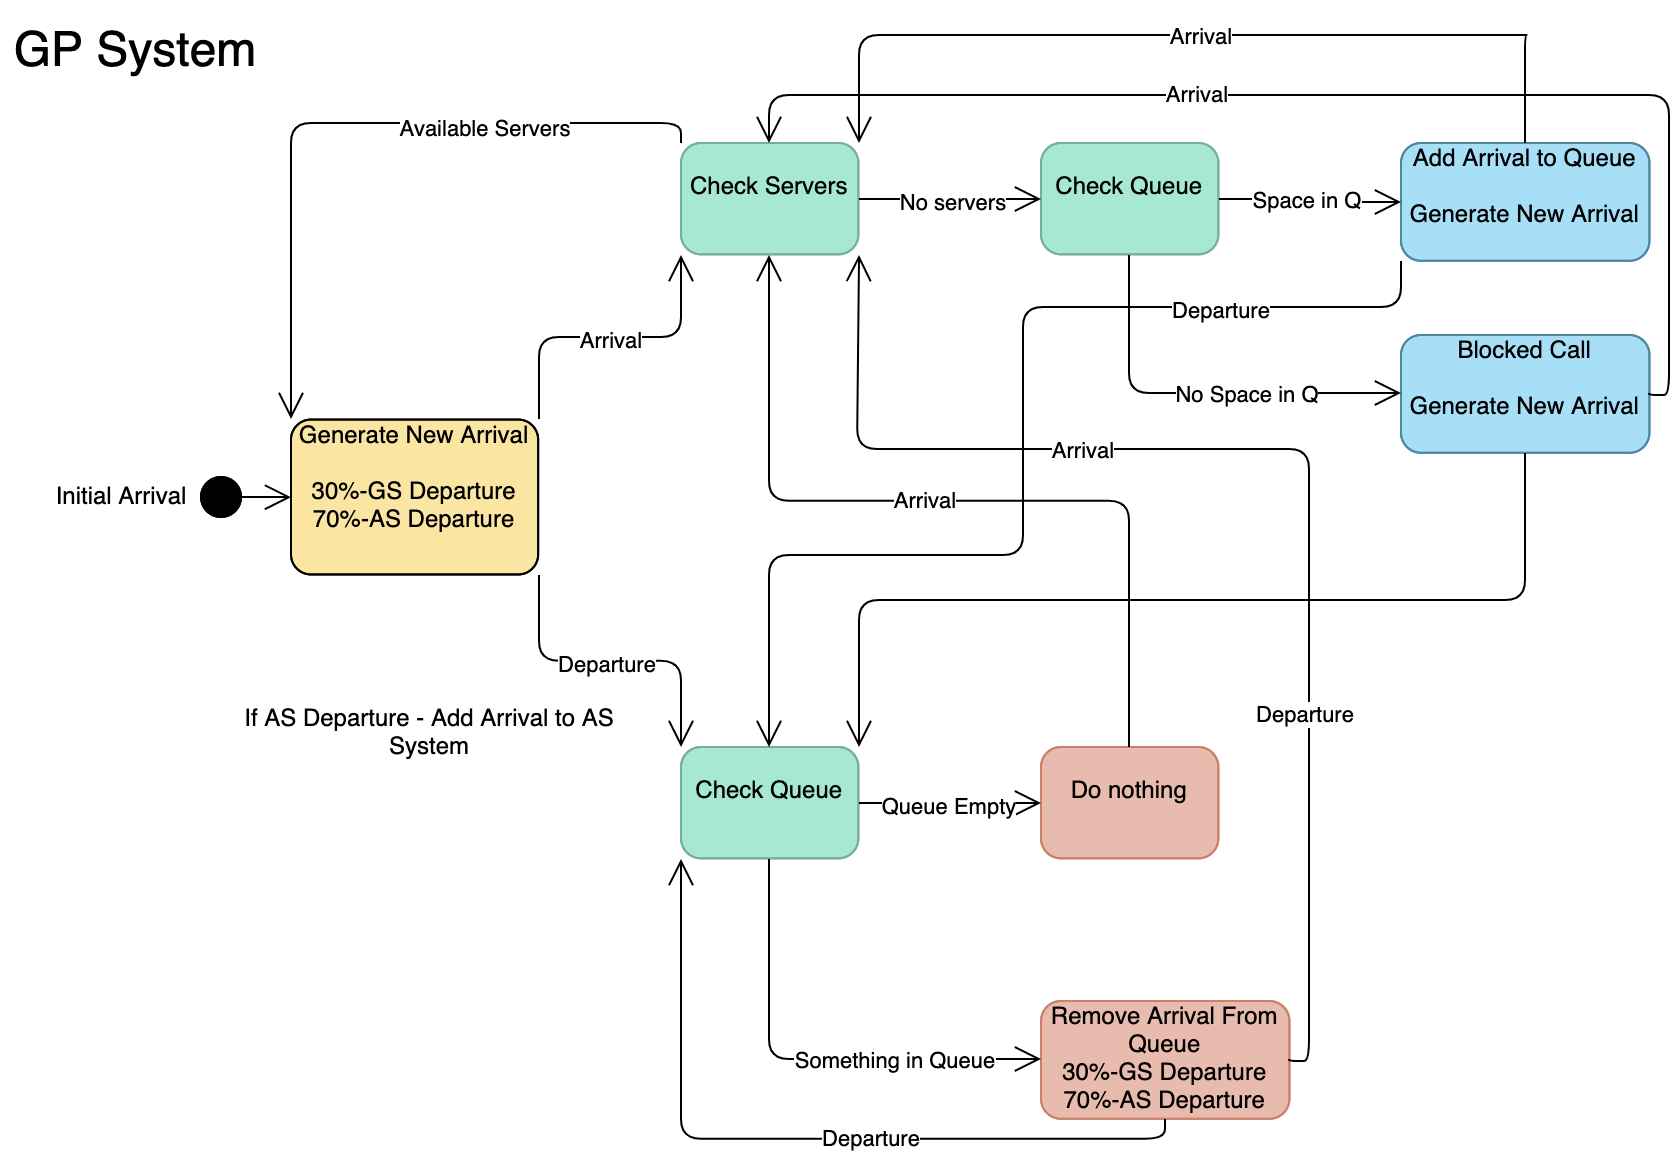
\includegraphics[width=.9\linewidth]{figs/intro/sm_gp.png}
    \caption{Máquina de estados do Sistema General Purpose}
    \label{fig:sm_gp}
\end{figure}

A figura \ref{fig:sm_gp} é uma máquina de estados que representa o algoritmo do \textbf{sistema GP}.
Primeiro verifica-se o tipo de evento que está na \textbf{lista\_eventos\_gp}.

Se o evento for de \textbf{CHEGADA}, verifica-se o estado do sistema.
Se os servidores estivem ocupados, verifica-se a fila de espera.
Se esta estiver livre, esse evento é colocado na \textbf{lista\_espera\_gp}.
Caso contrário é bloqueado.
Novas \textbf{CHEGADAS} são sempre geradas quando se processa uma \textbf{CHEGADA}.

Se o evento for de \textbf{PARTIDA}, verifica-se se há algum evento na \textbf{lista\_espera\_gp}.
Se houver, começa-se imediatamente a processar esse evento, gerando uma nova \textbf{PARTIDA}.
Caso contrário, passa-se para o próximo evento na \textbf{lista\_eventos\_gp}.

Por fim, considera-se que uma \textbf{CHEGADA} é gerada no \textbf{sistema AS} quando é processada uma \textbf{PARTIDA\_AS}.


\noindent
\newline
O princípio de funcionamento do sistema AS é semelhante, ilustrado na figura \ref{fig:sm_as}. Destaca-se alguma diferenças.


As \textbf{CHEGADAS} não são geradas no \textbf{sistema AS}, mas sim no \textbf{sistema GP}, pelo que o sistema pode ficar inativo, algo que não acontece com o \textbf{sistema GP}.
Além disso, não existe a risco de uma chamada ser bloqueada pois a fila é infinita.
A \textbf{lista\_eventos\_as} é constantemente verificada para detetar se alguma chamada foi reencaminhada para ser atendida pela sistema. Quando o sistema fica \textit{idle}, volta a este estado.

As \textbf{PARTIDAS} são geradas também quando uma CHEGADA é processada, no entanto a distribuição temporal é diferente das duas partidas do sistema GP.

\begin{figure}[H]
    \centering
    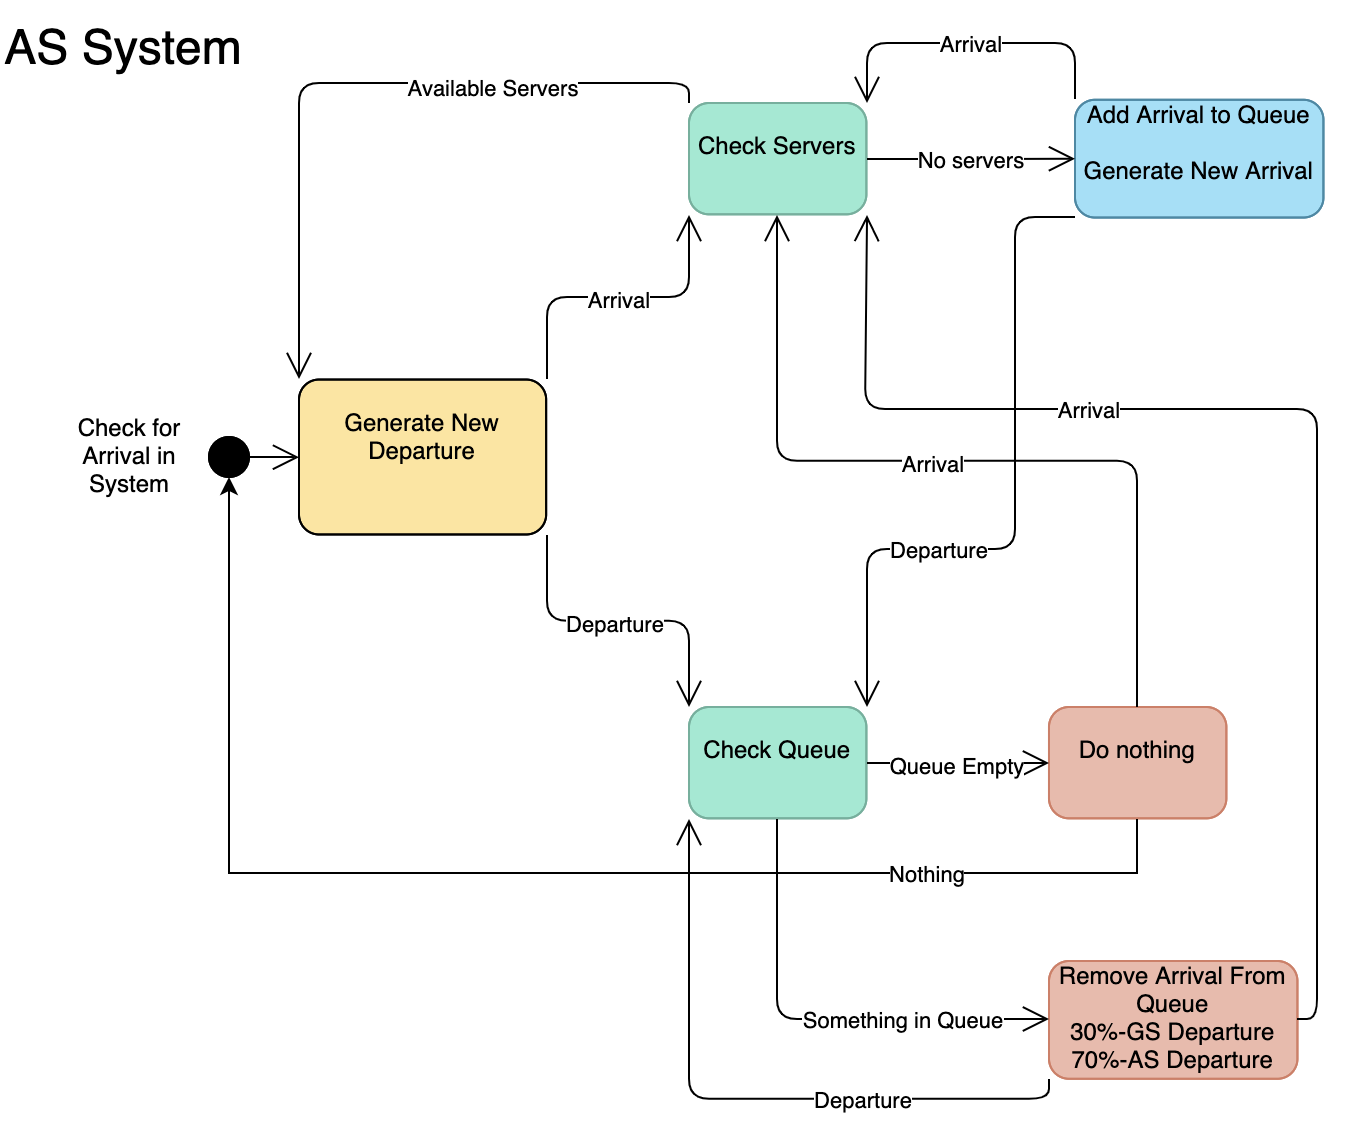
\includegraphics[width=.7\linewidth]{figs/intro/sm_as.png}
    \caption{Máquina de estados do Sistema Area Specific}
    \label{fig:sm_as}
\end{figure}

\section*{Estimativa do tempo de espera}

De forma a puder fornecer uma previsão do tempo de espera a cada chamada que chega, é necessário adotar um algoritmo de \textit{running average}.
Este algoritmo permite o calculo dinâmico da média do tempo de espera a cada chamada que chega, atualizando a cada iteração.

A estimativa do tempo de espera começa a 1. Quando uma chamada chega, duas situações podem acontecer:
\begin{itemize}
    \item Chamada é imediatamente atendida, pelo que o delay é 0 segundos.
    \item Chamada é colocada na fila de espera. O delay é calculado no momento em que a chamada sai da fila de espera.
\end{itemize}

Quando um novo valor de delay é obtido, uma nova média é calculada.
Por exemplo, com um delay de 60 segundos, a nova média será $\frac{0+60}{2}=30s$.
Quando uma nova chamada chegar, a estimativa de tempo de espera apresentada será de 30 segundos.
A cada iteração, este valor é atualizado.
Como este sistema tende para a estabilidade, este valor aproxima-se para um valor constante, que vai fornecer uma previsão mais sólida quantas mais chamadas forem atendidas.


\section*{Resultados da simulação}

De modo a garantir os objetivos de performance mínimos, necessitamos de pelo menos \textbf{4 Servidores GP}, \textbf{2 Servidores AS} e \textbf{Fila de Espera GP de tamanho 2}.
Os seguintes parâmetros foram obtidos:
\begin{center}
    \begin{tabular}{||c|c c||} 
    \hline
    Parâmetro & Mínimo & \textbf{Obtido} \\
    \hline\hline
    Delay Prob & 30\% & \textbf{12.83\%}\\ 
    \hline
    Blocked Prob & 2\% & \textbf{1.35\%}\\
    \hline
    Avrg Delay GS& 30s & \textbf{23.4s}\\
    \hline
    Avrg Delay Total & 60s & \textbf{24s} \\
    \hline
   \end{tabular}
\end{center}

O \textit{Bottleneck} deste sistema é o \textbf{Avrg Delay GS}, que está muito mais próximo do limite do que os restantes parâmetros.
Um relaxamento deste parâmetro para 40 segundo permitia que fosse utilizado apenas 3 servidores GP.

Com estes parâmetros, foram gerados histogramas que representam a distribuição dos atrasos e dos erros de previsão.

\begin{figure}[H]
    \centering
    \begin{subfigure}[b]{0.49\textwidth}
        \centering
    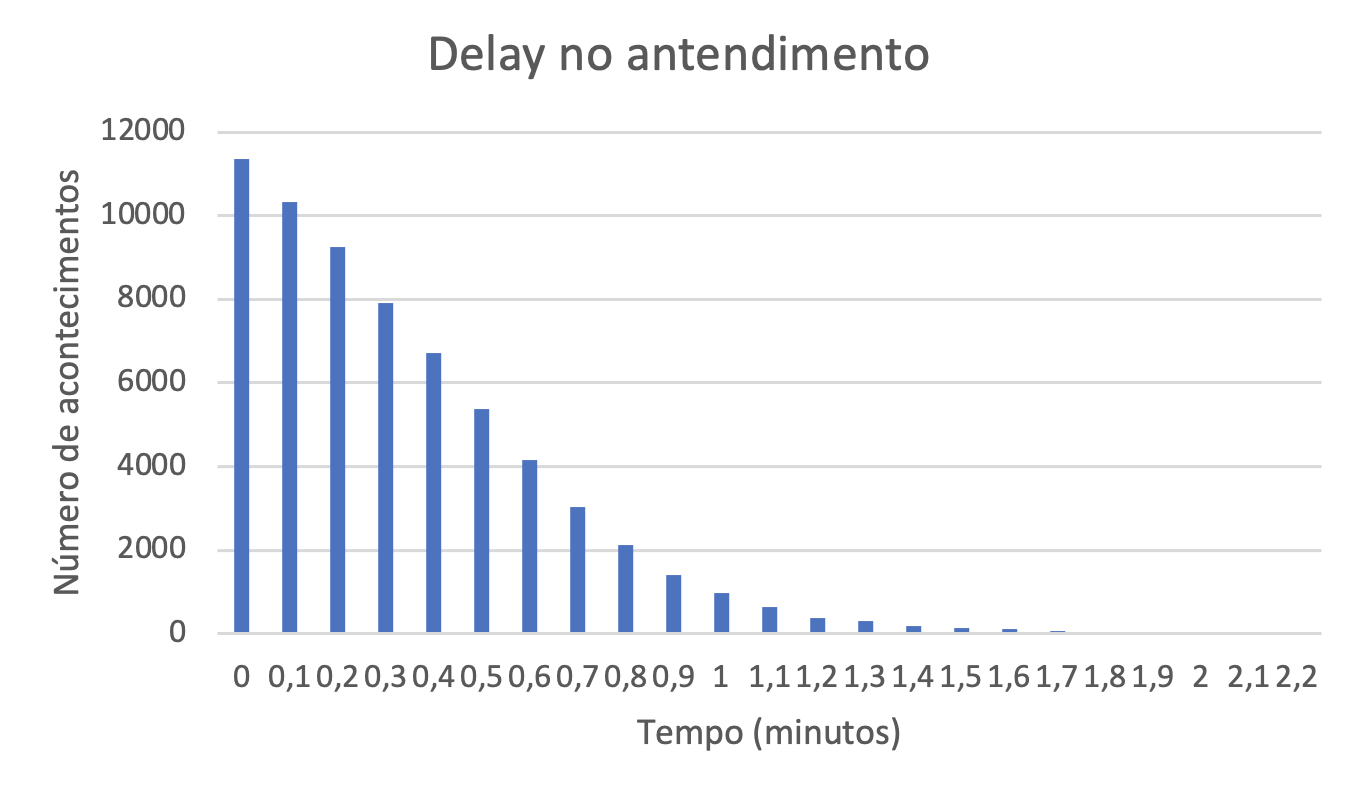
\includegraphics[width=\linewidth]{figs/intro/histo_delay.png}
    \caption{Distribuição dos delays no sistema}
    \label{fig:histo_delay}
    \end{subfigure}
    \hfill
    \begin{subfigure}[b]{0.5\textwidth}
        \centering
    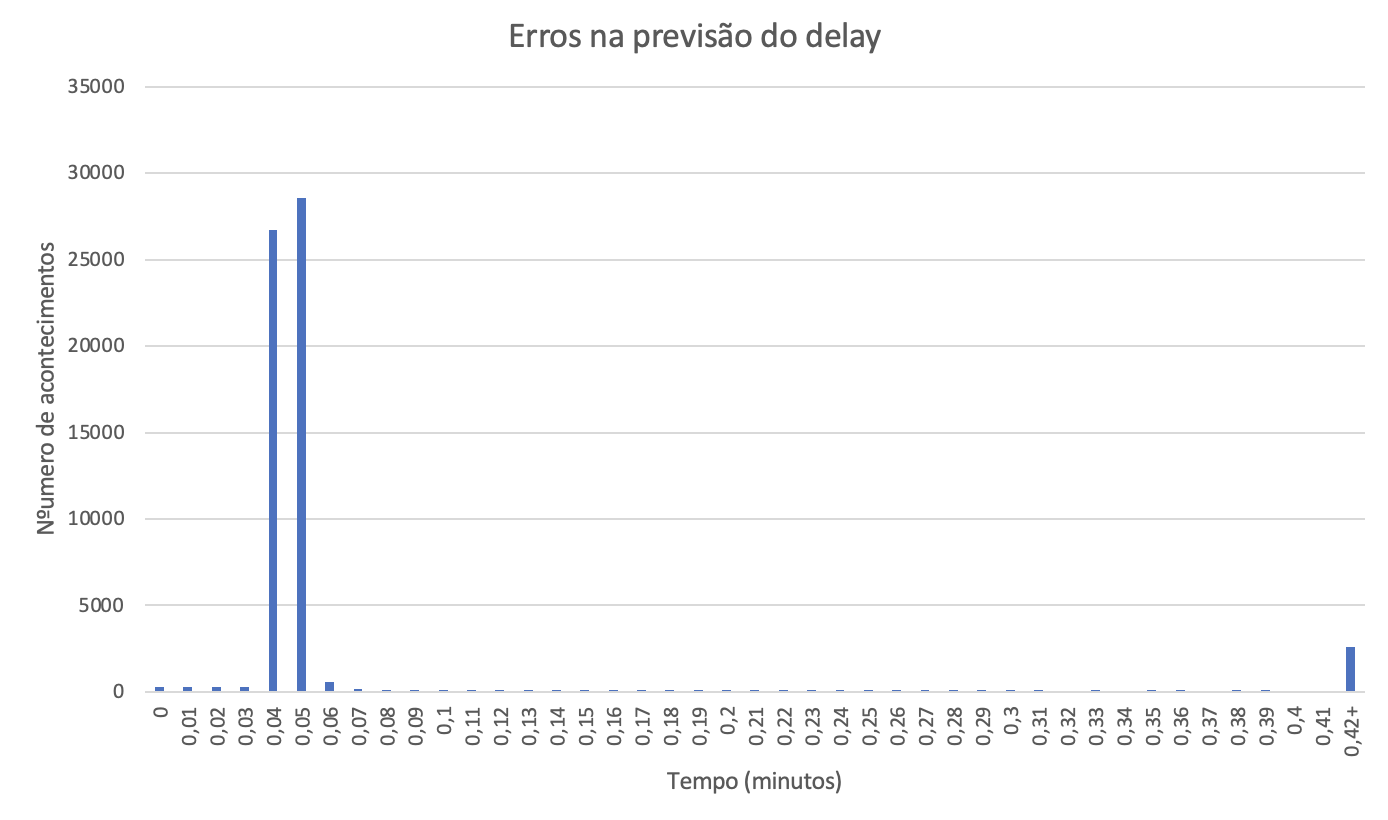
\includegraphics[width=\linewidth]{figs/intro/histo_erro.png}
    \caption{Distribuição do erro de previsão no sistema}
    \label{fig:histo_erro}
    \end{subfigure}
       \label{fig:histogramas}
\end{figure}

A distribuição dos dos \textit{Delays} aproxima-se de uma distribuição exponencial, pois este sistema é estável, ou seja, $\rho<1$.
Se $\rho>1$, esta distribuição seria crescente pois o tempo de espera iria aumentar com o tempo. Os delays 0 não estão representados.

Uma analíse do histograma dos erros indica que grande parte dos erros foi na ordem dos 0.04-0.06 segundos, que é sensivelmente o valor médio de atraso.
Mais uma vez, o facto do sistema ser estável fez com que os erros obtidos fossem da ordem da média.

\section*{Análise de Sensibilidade e Estimador}

\begin{figure}[H]
    \begin{floatrow}
    \ffigbox{%
    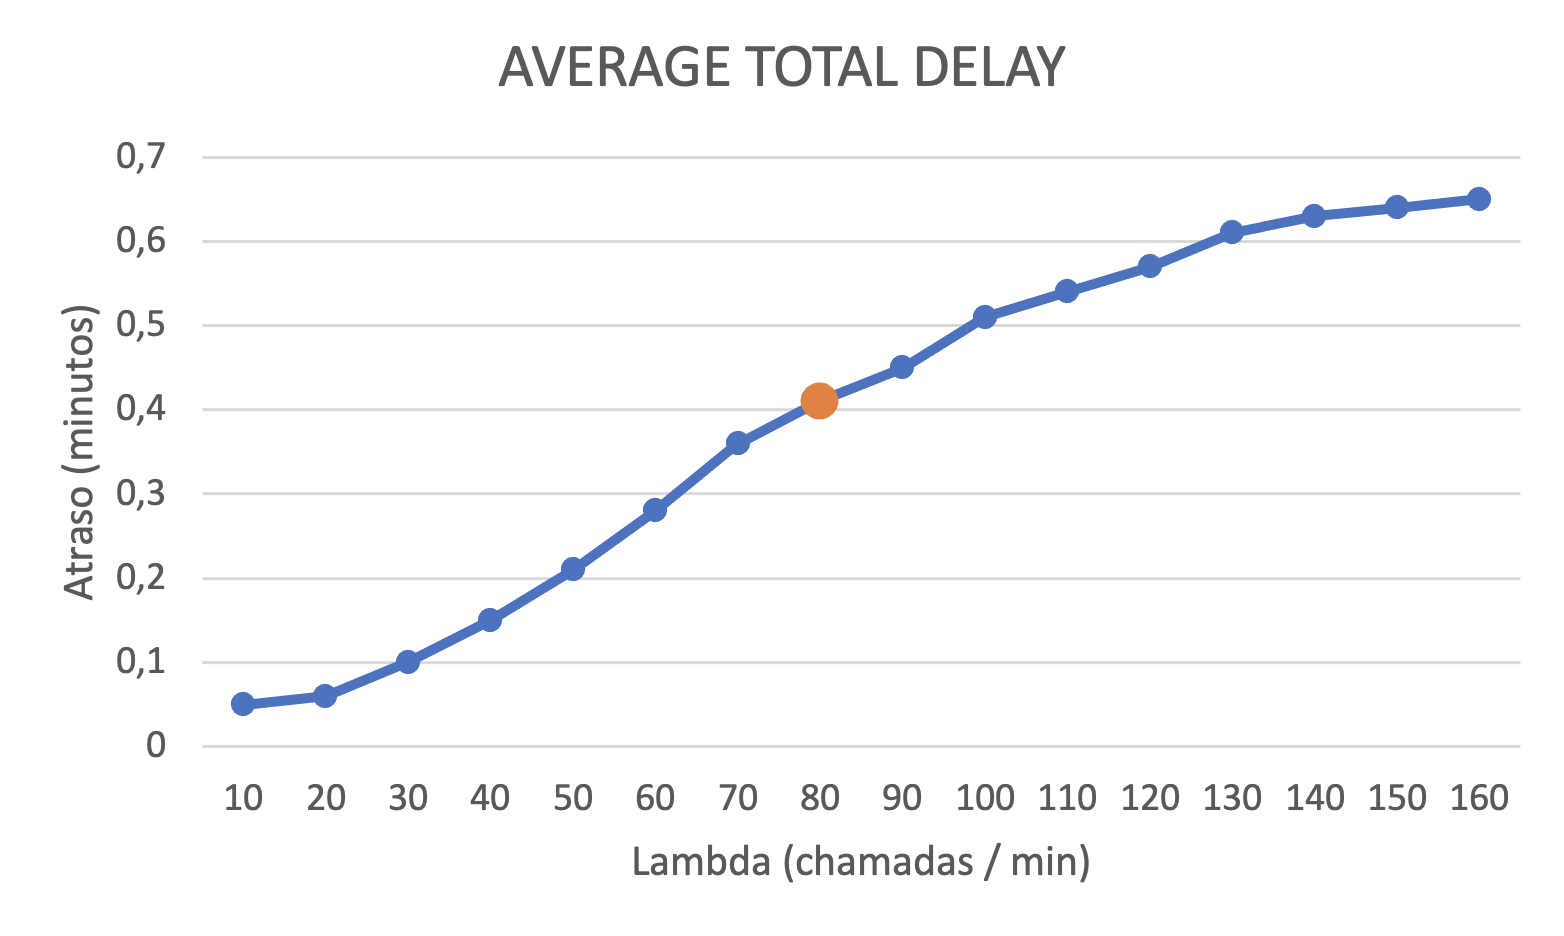
\includegraphics[width=.9\linewidth]{figs/intro/total_delay.png}
    }{%
    \caption{Total Delay time com variação da frequência de chegadas}
    }
    \capbtabbox{%
    \begin{tabular}{||c|c||} 
        \hline
        Intervalo de Confiança & 90\% \\
        \hline
        Número de Amostras & 30 \\
        \hline
        Graus de Liberdade & 29 \\
        \hline
        t (Student) & 1.6973 \\
        \hline
        Média & 0.410105 \\
        \hline
        Desvio Padrão & 0.005534535\\
        \hline
        Limite Inferior & 0.408389941 \\
        \hline
        Limite Superior & 0.411820059 \\
        \hline
       \end{tabular}
    }{%
    \caption{Estimador do Average Total Wait Time com intervalo de confiança de 90\% - 2 Tail}
    }
    \end{floatrow}
\end{figure}


A figura 4 mostra a relação entre a \textit{Arrival Rate} e o Atraso do sistema.
Observamos, como esperado, que o atraso tende para 0 à medida que se diminúi a \textit{Arrival Rate}.

À medida que o valor aumenta, o atraso tendo para um valor próximo de 0.65 minutos.
Isto deve-se ao facto da fila de espera ter tamanho limite.
O tempo que uma chamada tem que esperar se estiver no fim da fila não aumenta pois tem sempre o mesmo número de chamadas à sua frente.
O que aumenta é a probabilidade de perder a chamada. É deste modo de esperar este comportamento.

Também foi calculado um estimar para o Average Total Wait Time com base em 30 amostras do parâmetro.


\chapter{Setup}
Neste capítulo vamos abordar o setup de teste que foi utilizado neste trabalho e como foram configuradas as diferentes ferramentas,
nomeadamente o Apache e o Squid Cache.

\section{Servers HTTP}

\subsection{Apache}
Neste trabalho é necessário configurar dois websites dinâmicos que vão depois ser acedidos. E necessário que se gerem logs de acesso que irão
futuramente ser analisados. Neste sentido, foi utilizada a ferramenta sugerida pelo docente, o Apache.

O Apache é um servidor httpd open-source que permite dar deploy de uma forma simples a sites web a partir do computador do utilizador.
No nosso caso, configuramos dois websites, intuitivamente apelidados de site1 e site2, que foram alojados no tux 13 (172.16.1.13).
O primeiro site está designado à porta 80, porta \textit{default} para acessos HTTP, e o segundo na porta 81.

Desta forma, para aceder aos websites basta colocar no browser de um computador na mesma rede (irá ser abordado em \ref{proxy})
o IP 172.16.1.13 e 172.16.1.13:81 respetivamente. Note-se que se coloca ":81" para forçar o browser a aceder por essa porta. 
Caso contrário, iria optar pela porta predefinida para HTTP.

\subsection{Dynamic Update}
Hoje em dia é comum implementações de serviços de cache que guardam informação num servidor mais próximo do utilizador,
muitas vezes no próprio computador. Este serviço serve para diminuir a carga no \textit{host} do website.
Apesar de ser útil em contexto real, neste trabalho não o é pois impede o registo de todos os acessos aos websites.
Desta forma, os sites são carregados com conteúdo dinâmico que obriga sempre a aceder ao site através do seu \textit{host}.
Foi utilizado o code snippet fornecido pelo docente programado em PHP, pelo que foi necessário ativar esta ferramenta no Apache.

\subsection{Logging}
Tal como indicado previamente, o Apache permite o registo em \textit{logs} dos acessos feitos aos websites.
Estes logs são cruciais pois vão ser analisados futuramente em \ref{test}. Foram criados dois diretórios diferentes para cada site, 
cada um contendo o respetivo \textit{access.log} e \textit{error.log}. 

\section{Proxy HTTP} \label{proxy}

\subsection{Squid Cache}

O Squid Cache é um proxy (com funcionalidades de cache) open-source que mais um vez permite alojar um proxy num \textit{host}.
Os acessos proxy são geralmente feitos através da porta 3128. Neste caso, o IP do computador a alojar o proxy é 192.168.109.11.
Por isso, para aceder ao proxy, basta escolhermos como IP do proxy 192.168.109.11:3128.

Uma outra funcionalidade do Squid neste trabalho prende-se a estrutura da rede em que este trabalho está a ser desenvolvido.
O servidor tux onde estão a ser alojados os websites é um subdomain de servidor de bancada onde está a ser alojado o proxy.
Desta forma, mesmo dentro do VPN institucional, o nosso computador pessoal não consegue aceder diretamente aos sites.
Para isso é preciso usar o Squid que funciona como um túnel. Desta forma, temos acesso direto aos websites a partir de um computador fora da rede dos tux.


\subsection{Logging}
Tal como o Apache, o Squid também mantém um registo de \textit{logs} com todos os acessos feitos pelo squid, incluíndo o IP de origem e de destino.
Estes logs irão ser futuramente analisados também.

\chapter {Nagios}

\textbf{Nagios Core} é uma ferramenta de monitorização de sistemas grátis e \textit{open-source} \cite{Nagios}.
É também oferecido um serviço pago Nagios XI, que é construído sobre o sistema \textit{core}.

Esta ferramenta permite a monitorização de vários serviços, atuando como um \textit{scheduler} que executa periodicamente testes para verificar o estado dos serviços e sistemas.
Estes testes são os \textbf{plugins}, \textit{scripts} maioritariamente Perl, executáveis, desenvolvidos quer internamente, quer pela comunidade.
Existem plugins para testar várias funcionalidades, desde o estado de um servidor HTTP à carga de utilização do CPU num servidor.

É disponibilizada uma interface Web, com recurso ao Apache, onde várias estatísticas são apresentadas para o utilizador, assim como alertas sobre sistemas que estejam \textit{down}.
É de notar que várias versões do \textit{frontend} são disponibilizadas, aumentando a capacidade de customização do sistema.

Todas as configurações são feitas através de ficheiros \textit{txt} no host do Nagios, pelo que não é possível configurar a ferramenta na sua interface Web.

\begin{figure}[H]
    \centering
    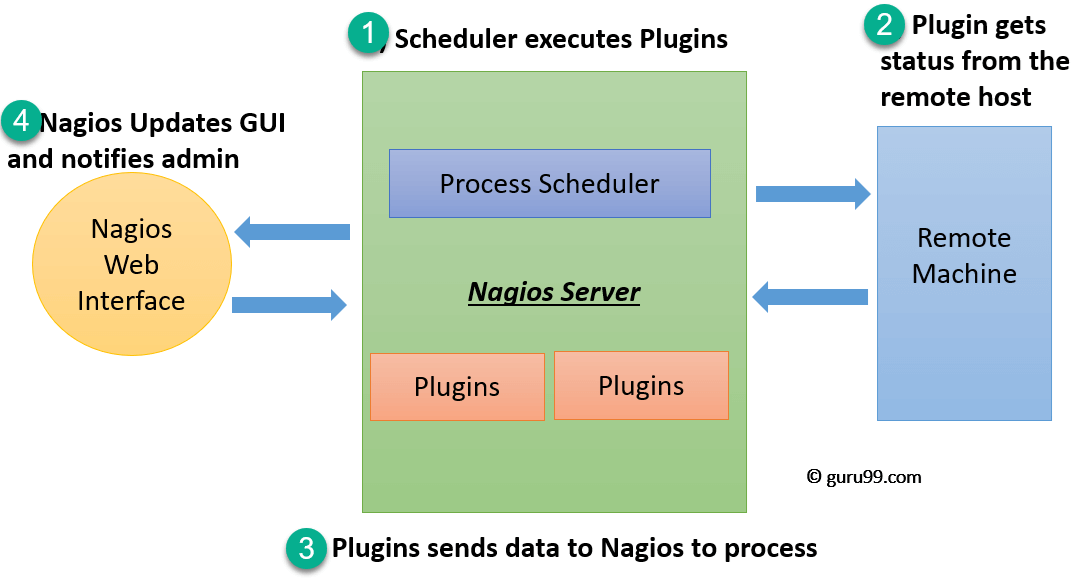
\includegraphics[width=.8\linewidth]{figs/nagios/nagios_wp}
    \caption{Princípio de funcionamento do Nagios}
    \label{fig:nagios_wp}
\end{figure}

\pagebreak

\section{Instalação e configuração}

A instalação foi feita segundo o guia de instalação do próprio Nagios \cite{Nagios_setup} no Tux13.
Foram definidos os dados de autenticação com o utilizador default \textit{nagiosadmin}.

Após a configuração inicial, foi feita a configuração dos sistemas.

O primeiro passo é importar os \textbf{Plugins} do Nagios.
Os seguintes \textit{packages} foram instalados no servidor:

\begin{itemize}
    \item nagios-plugins: os testes executáveis locais, i.e., que testam os serviços acedendo remotamente, por exemplo, a um servidor HTTP para verificar se está disponível.
    \item nagios-nrpe-plugins: os testes executáveis dos agentes, i.e., que são executados no sistema de destino para ter acesso a informação local, por exemplo, da utilização do CPU.
\end{itemize}

Devido aos objetivos deste trabalho consistirem maioritariamente com o teste dos serviços, foi utilizada a abordagem mais simples dos \textbf{nagios-plugins},
que não requer a instalação de agentes no computadores, apenas no servidor.

O segundo passo consiste em indicar ao Nagios quais os plugins utilizar e em que sistemas.
Para efeitos de simplificação, foi criada a pasta \verb|servers| no diretório \verb|/usr/local/nagios/etc/servers|.
Nesta pasta, foi criado um ficheiro .cfg para cada sistema, neste caso, \verb|tux12.cfg, localhost.cfg, tux13.cfg, router.cfg e switch.cfg|.

Nestes ficheiros é especificado quais são os plugins a executar em cada um dos computadores.
Por exemplo, o ficheiro \verb|tux12.cfg| ficou configurado da seguinte forma:

\pagebreak

\begin{lstlisting}
define host {
        use                          linux-server
        host_name                    tux12
        alias                        FTP-NTP-Mail
        address                      172.16.1.12
        register                     1
}

define service {

        use                     generic-service
        host_name               tux12
        service_description     Mail
        check_command           check_smtp
        notifications_enabled   1
}

define service {

        use                     generic-service
        host_name               tux12
        service_description     Ping
        check_command           check_ping
        notifications_enabled   1
}

define service {

        use                     generic-service
        host_name               tux12
        service_description     FTP
        check_command           check_ftp
        notifications_enabled   1
}
define service {

        use                     generic-service
        host_name               tux12
        service_description     NTP
        check_command           check_ntp_time
        notifications_enabled   1
}

define service {

        use                     generic-service
        host_name               tux12
        service_description     SSH
        check_command           check_ssh
}

\end{lstlisting}

Note-se que primeiro é feita uma definição do host e do respetivo IP.
Nos serviços, são identificados os testes a ser executados, especificando o host.
É possível definir todos os testes e hosts no mesmo ficheiro, mas tal não é boa prática pois torna-se muito difícil modificar as configurações do sistema.

\pagebreak

Dependendo do host e os serviços nele alojados, diferentes testes foram configurados:

\begin{table}[H]
    \begin{center}
        \begin{tabular}{ || c | c ||}
        \hline
        \textbf{Sistema} & \textbf{Testes}\\ 
        \hline
        Tux12 & \begin{tabular}{@{}c@{}}check\_ping \\ check\_ssh \\ check\_ntp \\ check\_ftp \\ check\_smtp (Mail)\end{tabular}\\
        \hline
        Tux14 & \begin{tabular}{@{}c@{}}check\_ping \\ check\_ssh \\ check\_http \\ check\_dns \\ check\_smtp (Mail)\end{tabular}\\
        \hline
        Router & \begin{tabular}{@{}c@{}}check\_ping \\ check\_snmp\_uptime\_v2 \\ \end{tabular}\\
        \hline
        Switch & \begin{tabular}{@{}c@{}}check\_ping \\ check\_snmp\_uptime\_v2 \\ \end{tabular}\\
        \hline
        Tux13 & localhost default tests \\
        \hline
        
        \end{tabular}
    \end{center}    
    \caption{Alocação dos serviços nos computadores}
    \label{tab:check_table}
\end{table}

Dois testes requereram mais atenção.

\textbf{Check\_dns}, apesar de ser um plugin instalado no \textit{package}, não está configurado no ficheiro \verb|commands.cfg|.
Este ficheiro é onde se define a sintax para correr os testes. Muitos já estão configurados, mas este não.
Desse modo configurou-se do seguinte modo:

\begin{lstlisting}

define command {
    command_name    check_dns
    command_line    $USER1$/check_dns -H $ARG1$ -s $HOSTADDRESS$ -a $ARG2$
}
\end{lstlisting}

com -H o endereço a fazer a \textit{query}, -s o servidor DNS a usar e -a o endereço IP esperado.
Os argumentos são passados quando se define o teste nos ficheiros de configuração.

\pagebreak

O teste predefinido do snmp, \textbf{check\_snmp}, não funcionou, pelo que instalou manualmente um novo script \textbf{check\_uptime} \footnote{\url{https://exchange.nagios.org/directory/Plugins/System-Metrics/Uptime/check_uptime--2F-check_snmp_uptime/details}}para o mesmo efeito.
Este script Perl for importado para a pasta \verb|\usr\lib\nagios\plugins|, sendo posteriormente definido como um executável para funcionar corretamente.
Este foi configurado do seguinte modo no ficheiro \verb|commands.cfg|:

\begin{lstlisting}

    define command {
        command_name check_snmp_uptime_v2
        command_line $USER1$/check_uptime.pl -2 -f -w -H $HOSTADDRESS$ -C public -T unix-sys
    }
\end{lstlisting}

Este comando retorna o OID \textbf{sysUpTime} do SNMP no sistema, verificando assim o seu funcionamento.

\section{Resultados}

\begin{figure}[H]
    \centering
    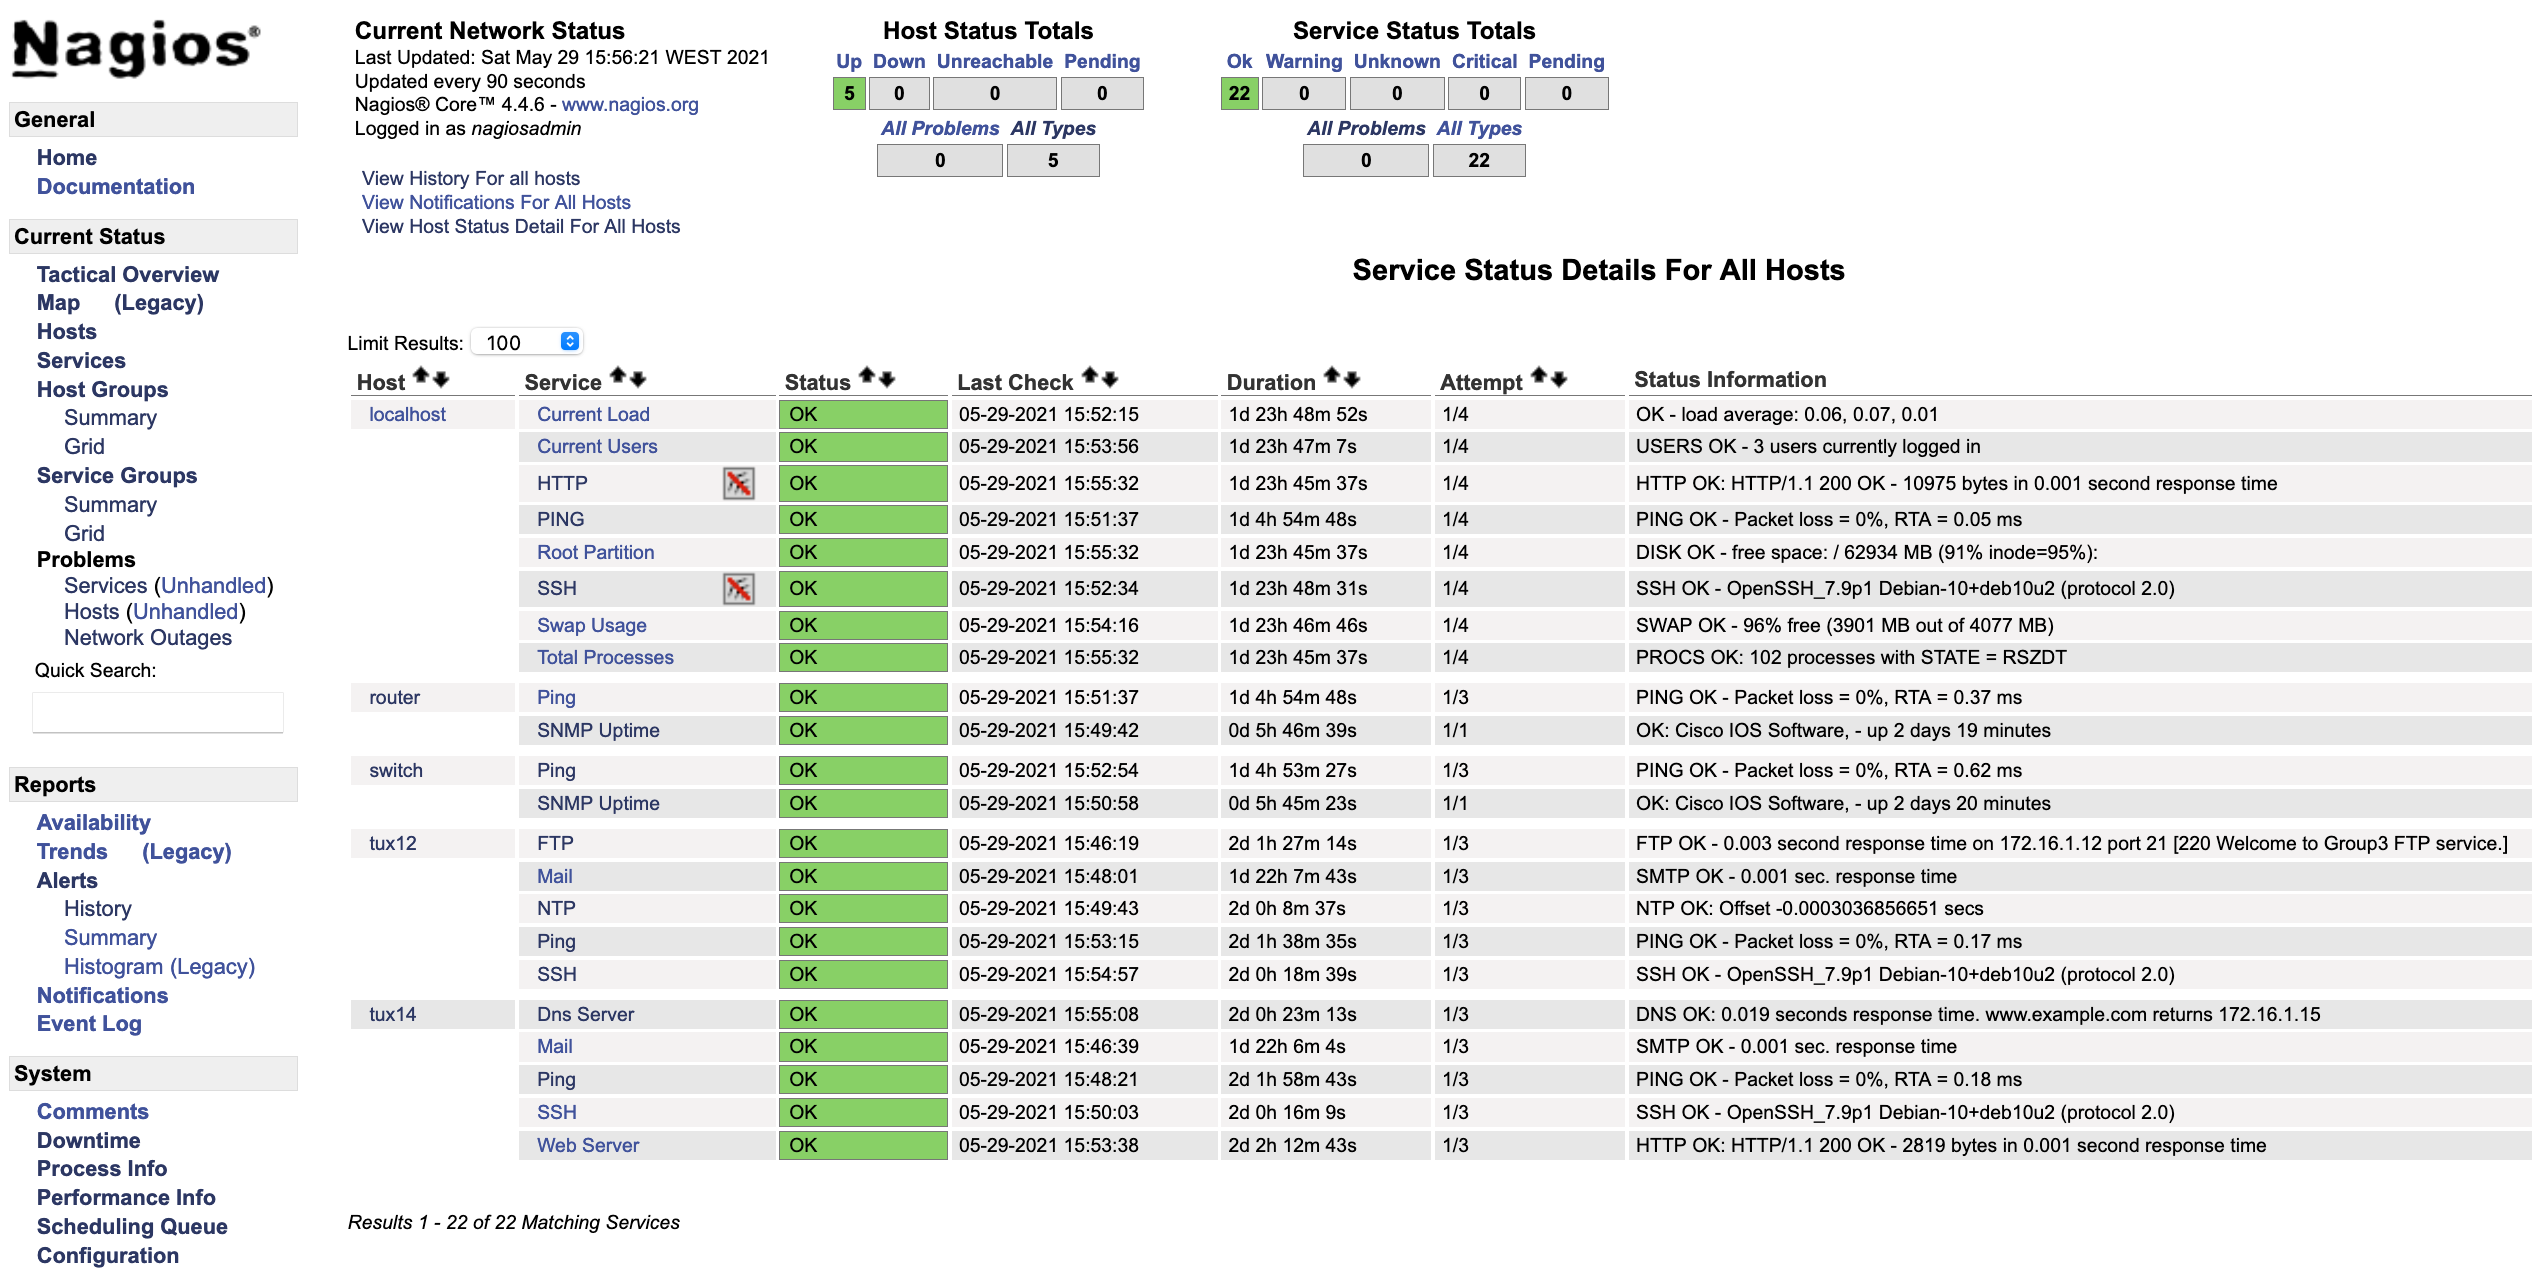
\includegraphics[width=.99\linewidth]{figs/nagios/nagios_web}
    \caption{Interface Web com o status dos serviços e hosts}
    \label{fig:nagios_web}
\end{figure}

Como observado, todos os serviços estão \textbf{OK}.
Também é apresentada informação relativamente ao \textit{uptime} dos serviços, assim como o retorno dos testes.

O campo \textbf{Last Check} indica quando foi executado o último teste.
É possível configurar o Nagios para aumentar a frequência de testes, no entanto isso aumenta também o tráfego interno de controlo pelo que é um \textit{trade-off} a ter em conta.

Clicando em cada serviço ou host, é possível obter informação mais específica.
No entanto, é uma \textit{frontend} bastante simples e intuitiva.

\pagebreak

\section{Teste de falhas}

Primeiramente, simulou-se falhas nos serviços, parando alguns processos nos Tuxs:

\begin{center}
    Tux12 \\
    \verb|systemctl stop vsftpd - Falha do servidor FTP| \\
    \verb|systemctl stop postfix - Falha do servidor Email| \\

    \vspace{1cm}
    Tux14 \\
    \verb|systemctl stop bind9 - Falha do servidor DNS| \\
    \verb|systemctl stop apache2 - Falha do servidor HTTP|
\end{center}

Após algum tempo de atualização de informação, o output da interface do Nagios foi o seguinte:

\begin{figure}[H]
    \centering
    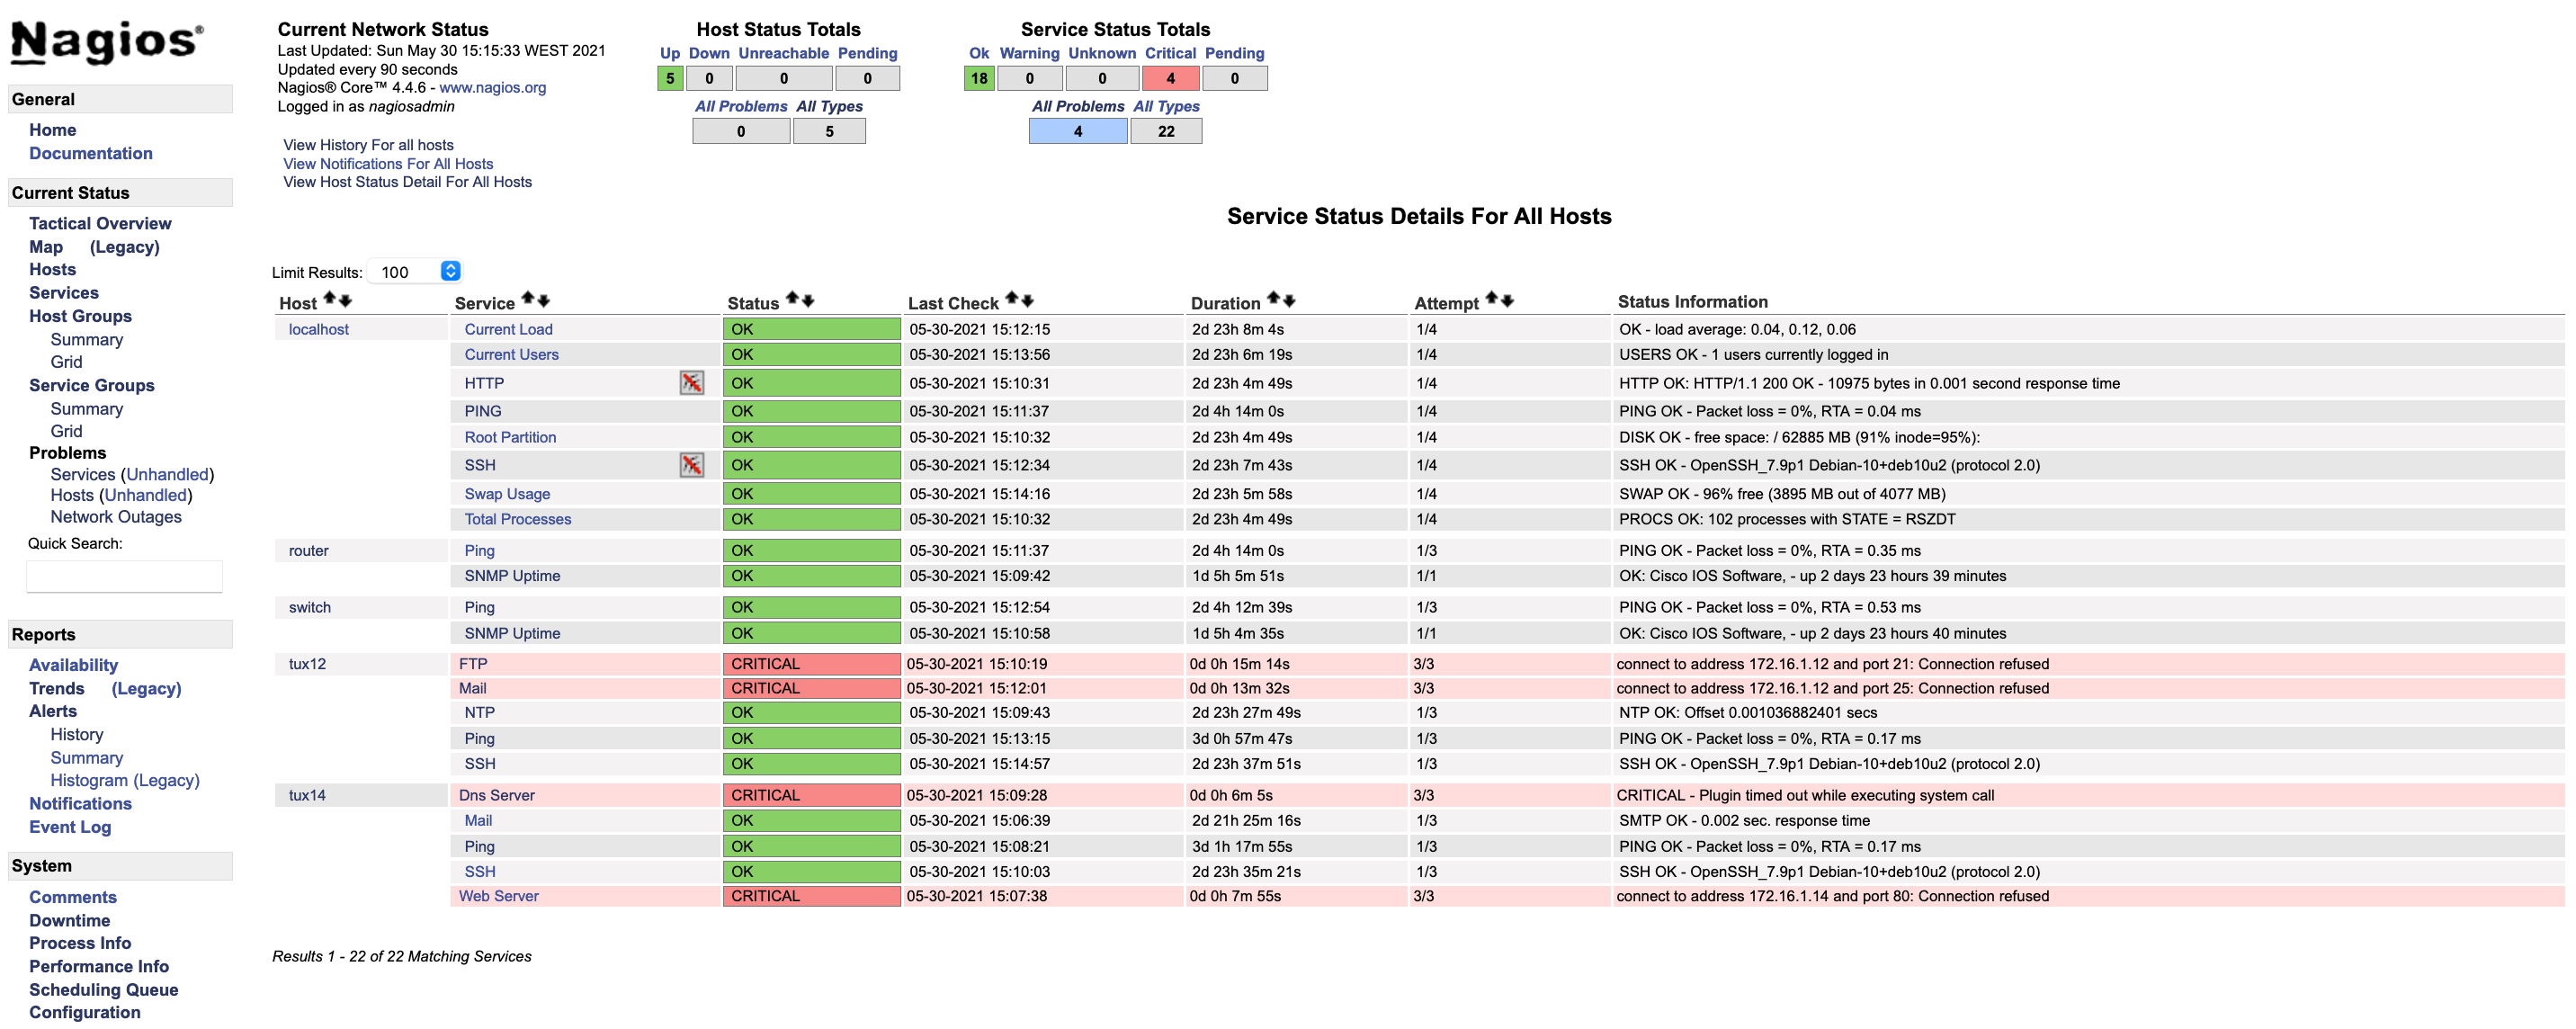
\includegraphics[width=\linewidth]{figs/nagios/nagios_errors}
    \caption{Falha de serviços}
    \label{fig:nagios_errors}
\end{figure}

Como se observa, os serviços desativados estão \textbf{CRITICAL}, sendo possível observar o output dos plugins.
É também apresentado quando tempo já passou desde que o serviço falhou.

De seguida simulou-se uma falha no Tux14.
Para se simular este evento, configurou-se dois \textit{cronjobs} consecutivos:
\begin{itemize}
    \item ifconfig eth0 down: cortar a ligação do Tux14 à rede
    \item ifconfig eth0 up: ativar novamente a interface para retomar o acesso 15 minutos depois do anterior
\end{itemize}

\begin{figure}[H]
    \centering
    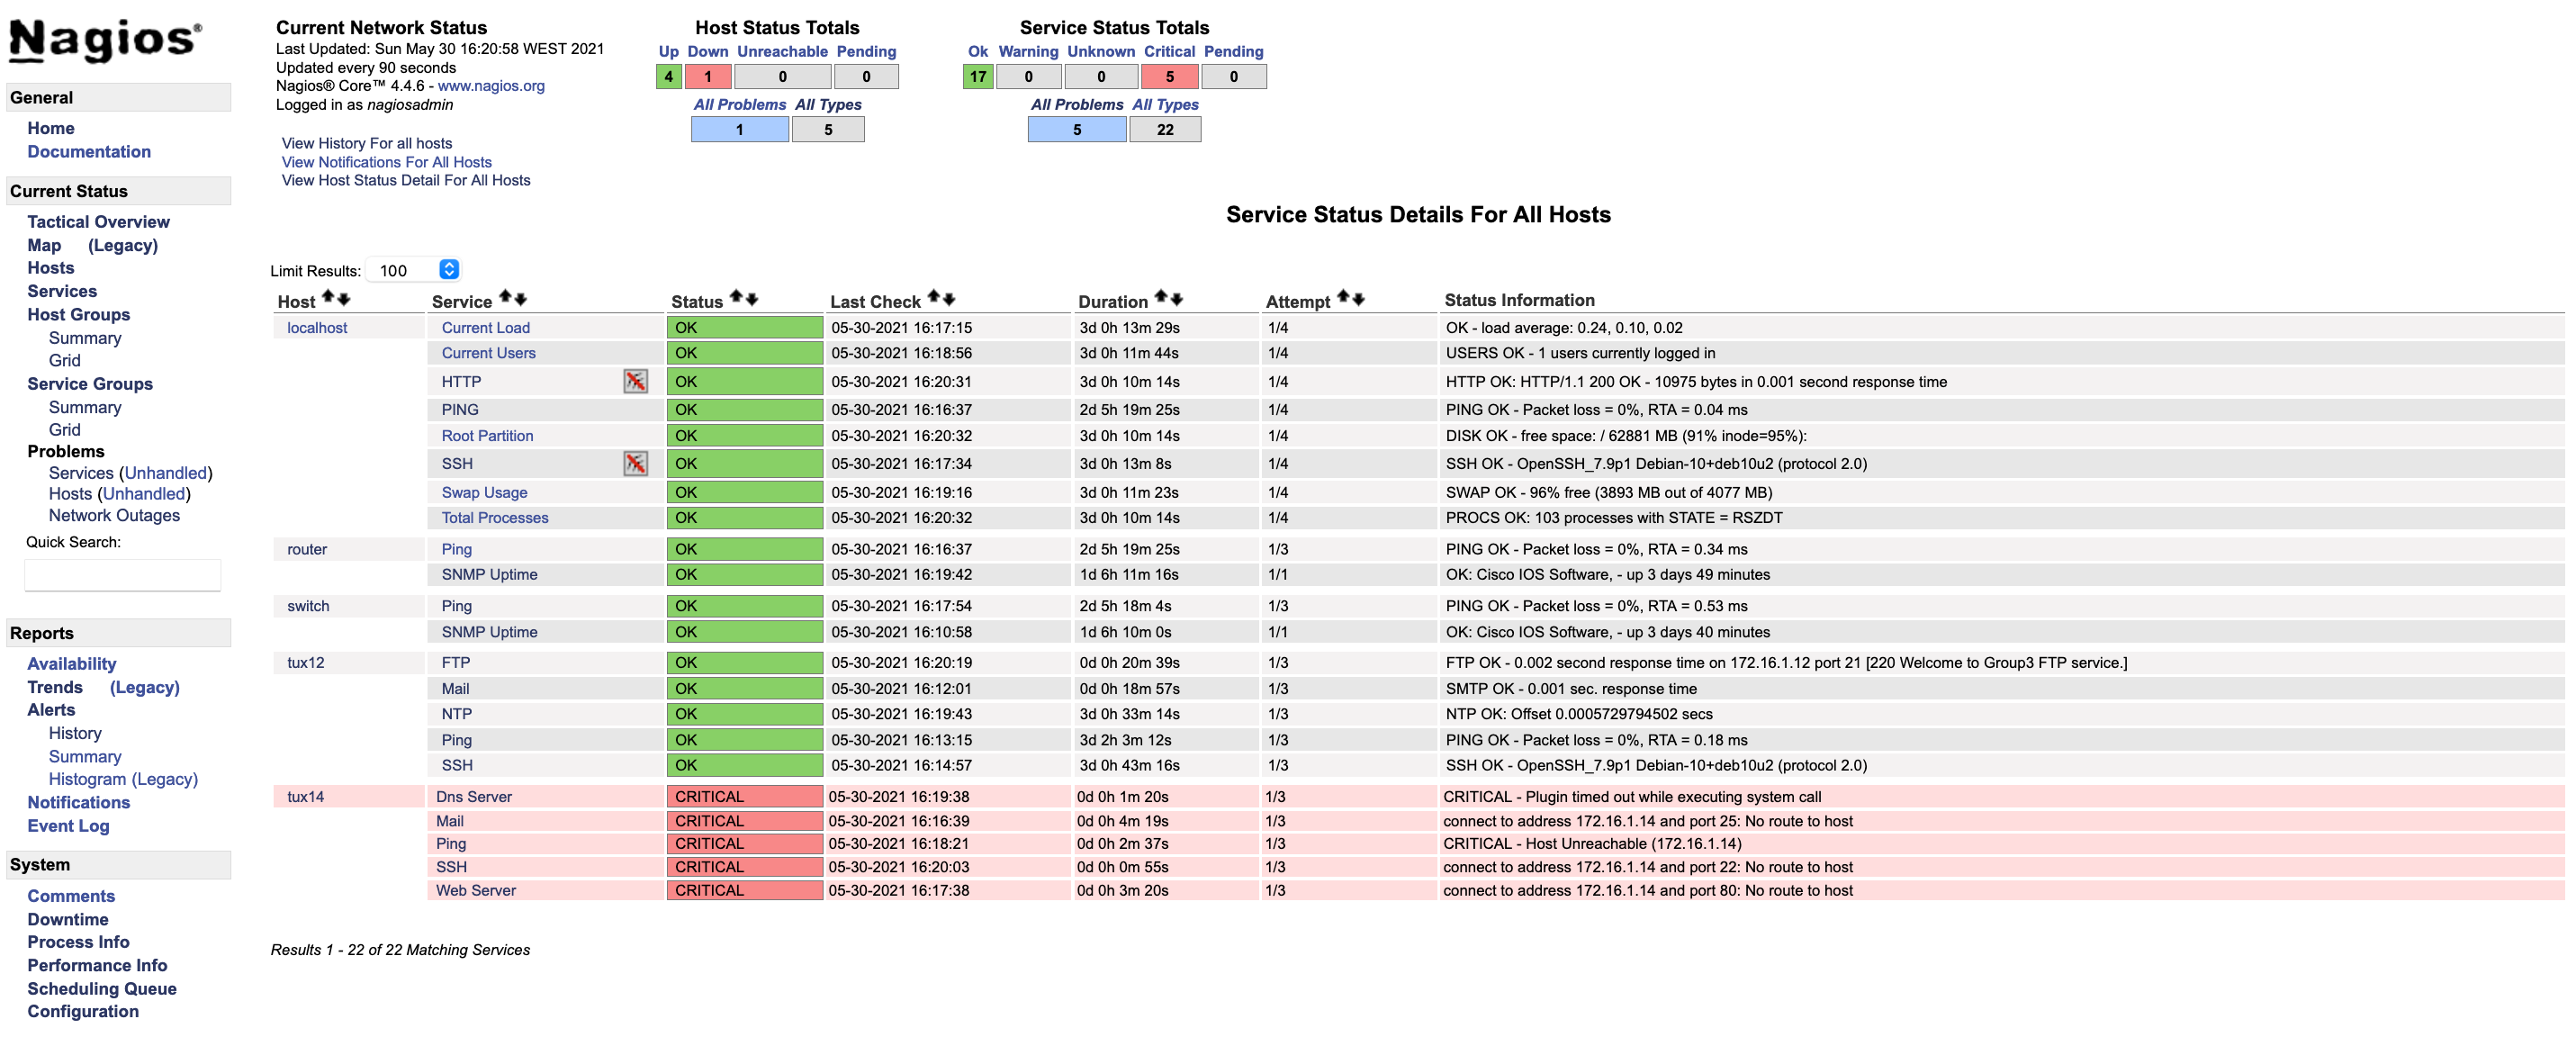
\includegraphics[width=\linewidth]{figs/nagios/nagios_tux14_down}
    \caption{Falha do Tux14}
    \label{fig:nagios_tux14_down}
\end{figure}

Neste cenário, não só estão os serviços no estado \textbf{CRITICAL}, mas também os testes de conectividade Ping e SSH.
O próprio host aparece a vermelho, e no topo da página é possível observar que há um host que está \textit{down}.

O Nagios demorou cerca de 1 minuto a detetar que host estava down, que está relacionado com a frequência do teste configurada.
\chapter{Zabbix}

\textbf{Zabbix}, tal como o Nagios Core, é uma ferramenta de monitorização de sistemas de rede e informação \textit{open-source} \cite{Zabbix}.
Permite a supervisão de diversos sistemas tais como redes, servidores VMs e serviços de cloud.
Paralelamente a estes serviços, é também possível monitorizar o estado hardware em sistemas onde o Zabbix esteja instalado.
O Zabbix funciona com apoio de uma base de dados. 
Se por predefinição, o Nagios usa MySQL, o Zabbix permite escolher de uma gama de opções, nomeadamente MySQL, MariaDB, PostgreSQL, etc.

O Zabbix não funciona à base de plugins, mas sim de \textbf{items}.
Este items têm o mesmo princípio de funcionamento, consistindo em testes executados periodicamente para monitorizar uma característica específica.
Os items podem ter outputs diferentes, quer seja números, strings ou booleanos.

No entanto, é de notar que o Zabbix não sabe interpretar o output destes items como correto ou não.
Para se definir o estado de um serviço ou \textit{feature}, é preciso definir os \textbf{triggers}.

Triggers correspondem a testes que são feitos ao output dos items.
Por exemplo, se um determinado item tem como output possível \textbf{1/0},
um trigger pode definir 1 como OK e 0 como ERROR, dando desse modo feedback ao utilizar sobre o estado de serviço de uma forma mais direta.

Para simplificar o processo de setup, e evitar a configuração manual de todos os items e correspondentes triggers,
são fornecidos \textbf{Templates} que contêm um conjunto de items e triggers adequados para determinados contextos.
Por exemplo, o template \textbf{Template App HTTP Service} contém um item que testa um servidor HTTP, e um trigger que processa o output para determinar o seu estado.
Alguns templates também contêm \textbf{dashboards}, que são uma compilação visual de informação relevante naquele template.

\pagebreak

\section{Instalação e configuração}

A instalação foi feita de acordo com a documentação do Zabbix \cite{Zabbix_setup} no Tux13.

Similarmente ao Nagios, o Zabbix oferece duas opções de monitorização:

\begin{itemize}
    \item Zabbix-agent: O Zabbix-agent é instalado no host destino, onde este coleta informação relevante do funcionamento do sistema, como a carga de CPU, disco, etc.
    O servidor Zabbix recebe depois esta informação diretamente do host, podendo assim mostrar várias estatísticas locais. É adequado quando queremos monitorizar um servidor ou computador.
    \item \textit{Agentless}: Os testes são feitos apenas sobre serviços que possam ser acedidos externamente, por exemplo, um servidor HTTP.
    Não é preciso instalar nada, sendo que a monitorização destes sistemas recorre a protocolos de comunicação como HTTP, SSH, SNMP, TELNET, etc. É adequado quando queremos monitorizar um componente de \textit{networking}, como um Router ou Switch.
\end{itemize}

Tendo isto consideração, a abordagem \textbf{Zabbix-agent} foi utilizada nos casos dos Tuxs, e a abordagem \textbf{Agentless} no Switch e no Router.

O próximo passo consiste na instalação dos diferentes \textit{packages} requeridos pelo Zabbix.
É aqui que se define também qual é a base de dados que se vai usar. A escolhida foi a \textbf{PostgreSQL}.

Foram definidos \textit{Users} e as respetivas \textit{passwords} quer para o Zabbix, quer para a base de dados.
O passo seguinte consiste na criação da base de dados que contém todas as configurações do Zabbix \footnote{A documentação online está errada a vários níveis, quer nos diretórios, quer na estrutura da base de dados.
No entanto a documentação fornecida localmente após a instalação do respetivo \textit{package} está correta}.

Após a configuração inicial, é definido no ficheiro \verb|/etc/zabbix/zabbix_server.conf| os parâmetros da base de dados criada:

\begin{lstlisting}
    DBHost= (string nula para o caso do PostgreSQL)
    DBName=zabbix
    DBUser=zabbix
    DBPassword=12345
\end{lstlisting}

Posteriormente, é feita a configuração final na página Web do Zabbix.
Após este passo, é possível iniciar a configuração da monitorização da rede.

A instalação dos agentes no Tux12, Tux13 e Tux14 é feita com a instalação do devido \textit{package}.
Posteriormente, o ficheiro \verb|/etc/zabbix/zabbix_agentd.conf| é modificado, especificando-se nas linhas “Server=” and “ServerActive=” o IP do servidor Zabbix.
O agente no Tux13 também é instalado pois é necessário para se poder fazer a monitorização do hardware do sistema no servidor.

\pagebreak

Ao contrário do Nagios, o Zabbix não é configurado localmente no sistema editando ficheiros de configuração, mas sim na interface Web do software.
Logo à partida, é possível afirmar que, para o utilizador comum, é mais fácil usar uma UI do que recorrer extensivamente ao terminal.

Os \textbf{Hosts} são a primeira coisa a definir.
A definição de um host consiste na definição da interface de comunicação entre o host e o servidor.
Além do IP, é preciso definir se esses hosts tem ou não agente.
No caso do Tux12 e Tux14, foi definida uma interface com agente.
No caso do Switch e do Router, foi definida uma interface com recurso ao protocolo SNMP.

\begin{figure}[H]
    \centering
    \begin{subfigure}[b]{0.9\textwidth}
        \centering
        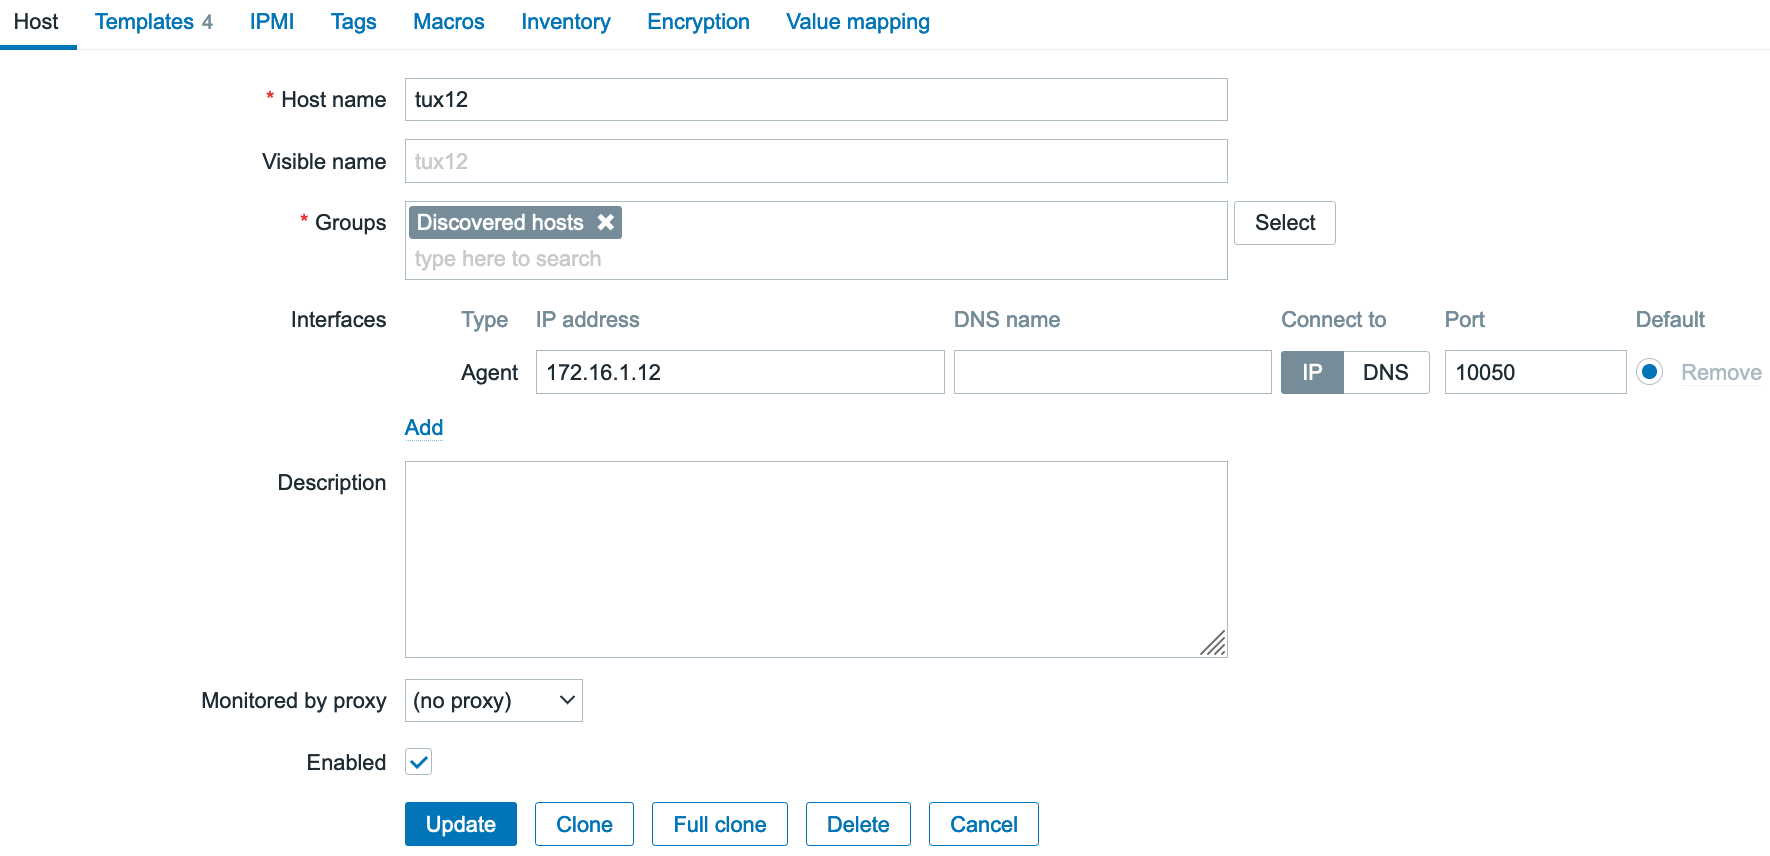
\includegraphics[width=.9\linewidth]{figs/zabbix/tux12_setup_1}
        \caption{Interface do Tux12 - Agent}
        \label{fig:tux12_setup_1}
    \end{subfigure}
    \hfill
    \begin{subfigure}[b]{0.9\textwidth}
        \centering
        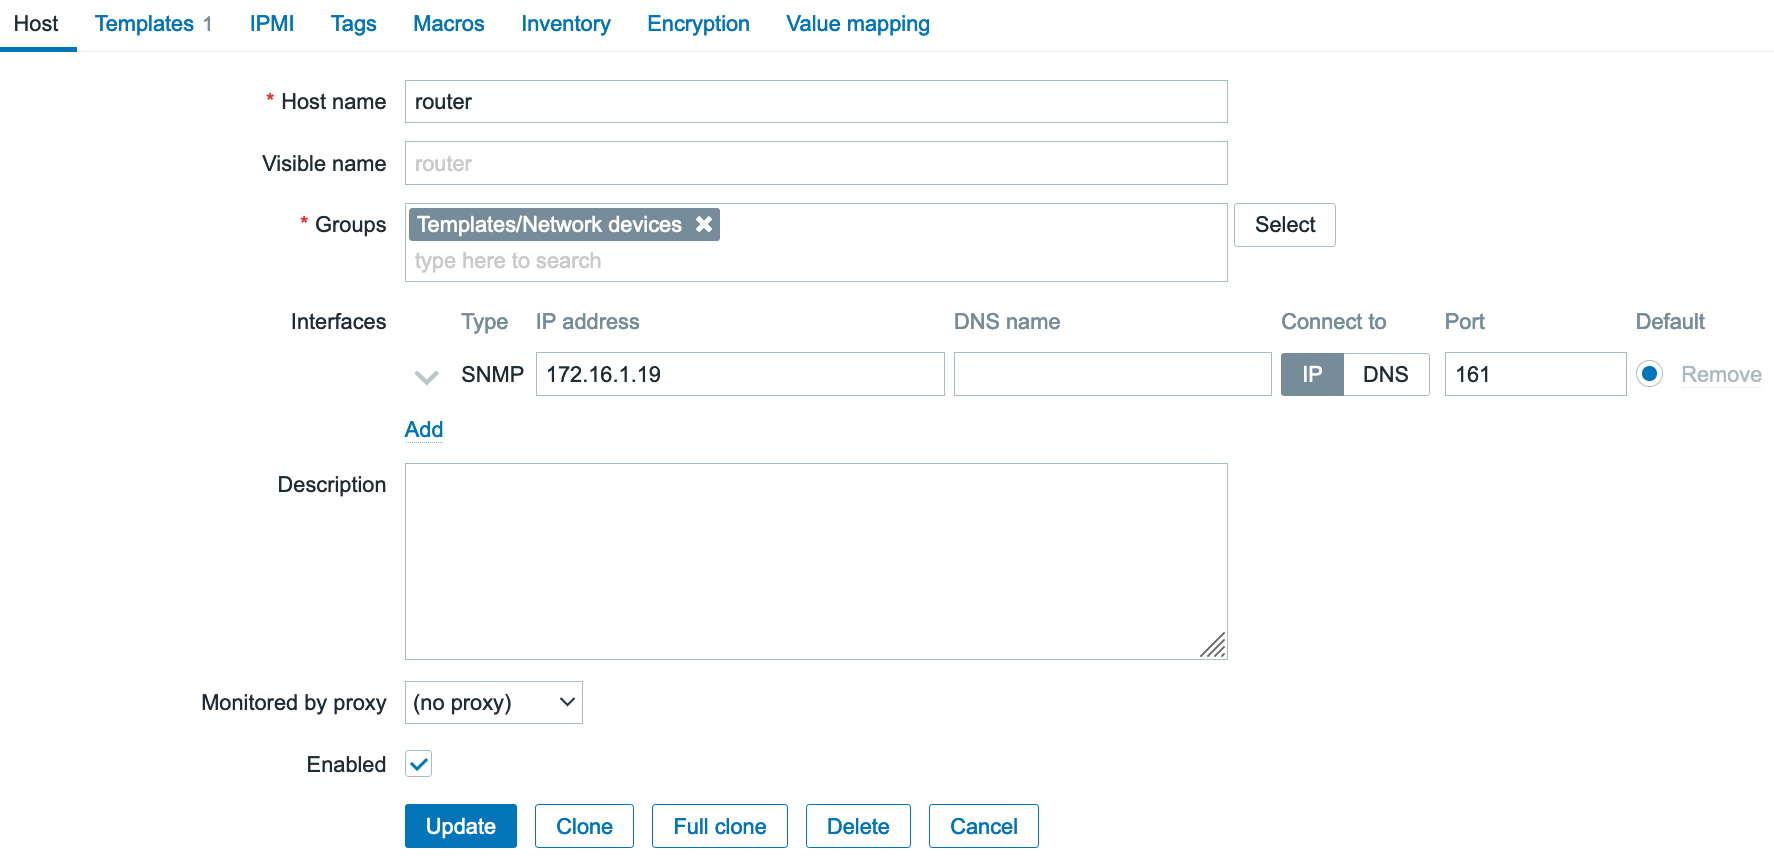
\includegraphics[width=.9\linewidth]{figs/zabbix/router_setup_1}
        \caption{Interface do Router - SNMP}
        \label{fig:router_setup_1}
    \end{subfigure}
    \caption{}
\end{figure}

Após se assegurar a comunicação entre os diferentes sistemas, é iniciada a configuração da monitorização dos diferentes serviços.

\pagebreak

Similarmente ao Nagios, e dependendo do hosts (Agent ou Agentless) e dos serviços nele alojados, os seguintes templates foram adicionados a cada um:

\begin{table}[H]
    \begin{center}
        \begin{tabular}{ || c | c ||}
        \hline
        \textbf{Sistema} & \textbf{Testes}\\ 
        \hline
        Tux12 & \begin{tabular}{@{}c@{}}Template App Zabbix Agent \\ Template App NTP Service \\ Template App FTP Service \\ Template App SMTP Service\end{tabular}\\
        \hline
        Tux14 & \begin{tabular}{@{}c@{}}Template App Zabbix Agent \\ Template App HTTP Service\\ Template App SMTP Service\end{tabular}\\
        \hline
        Router & Template Module Generic SNMPv2\\
        \hline
        Switch & Template Module Generic SNMPv2\\
        \hline
        Tux13 & \begin{tabular}{@{}c@{}}Template App Zabbix Server \\ Template App Zabbix Agent \\ \end{tabular}\\
        \hline
        
        \end{tabular}
    \end{center}    
    \caption{Alocação dos serviços nos computadores}
    \label{tab:template_table}
\end{table}


\begin{figure}[H]
    \centering
    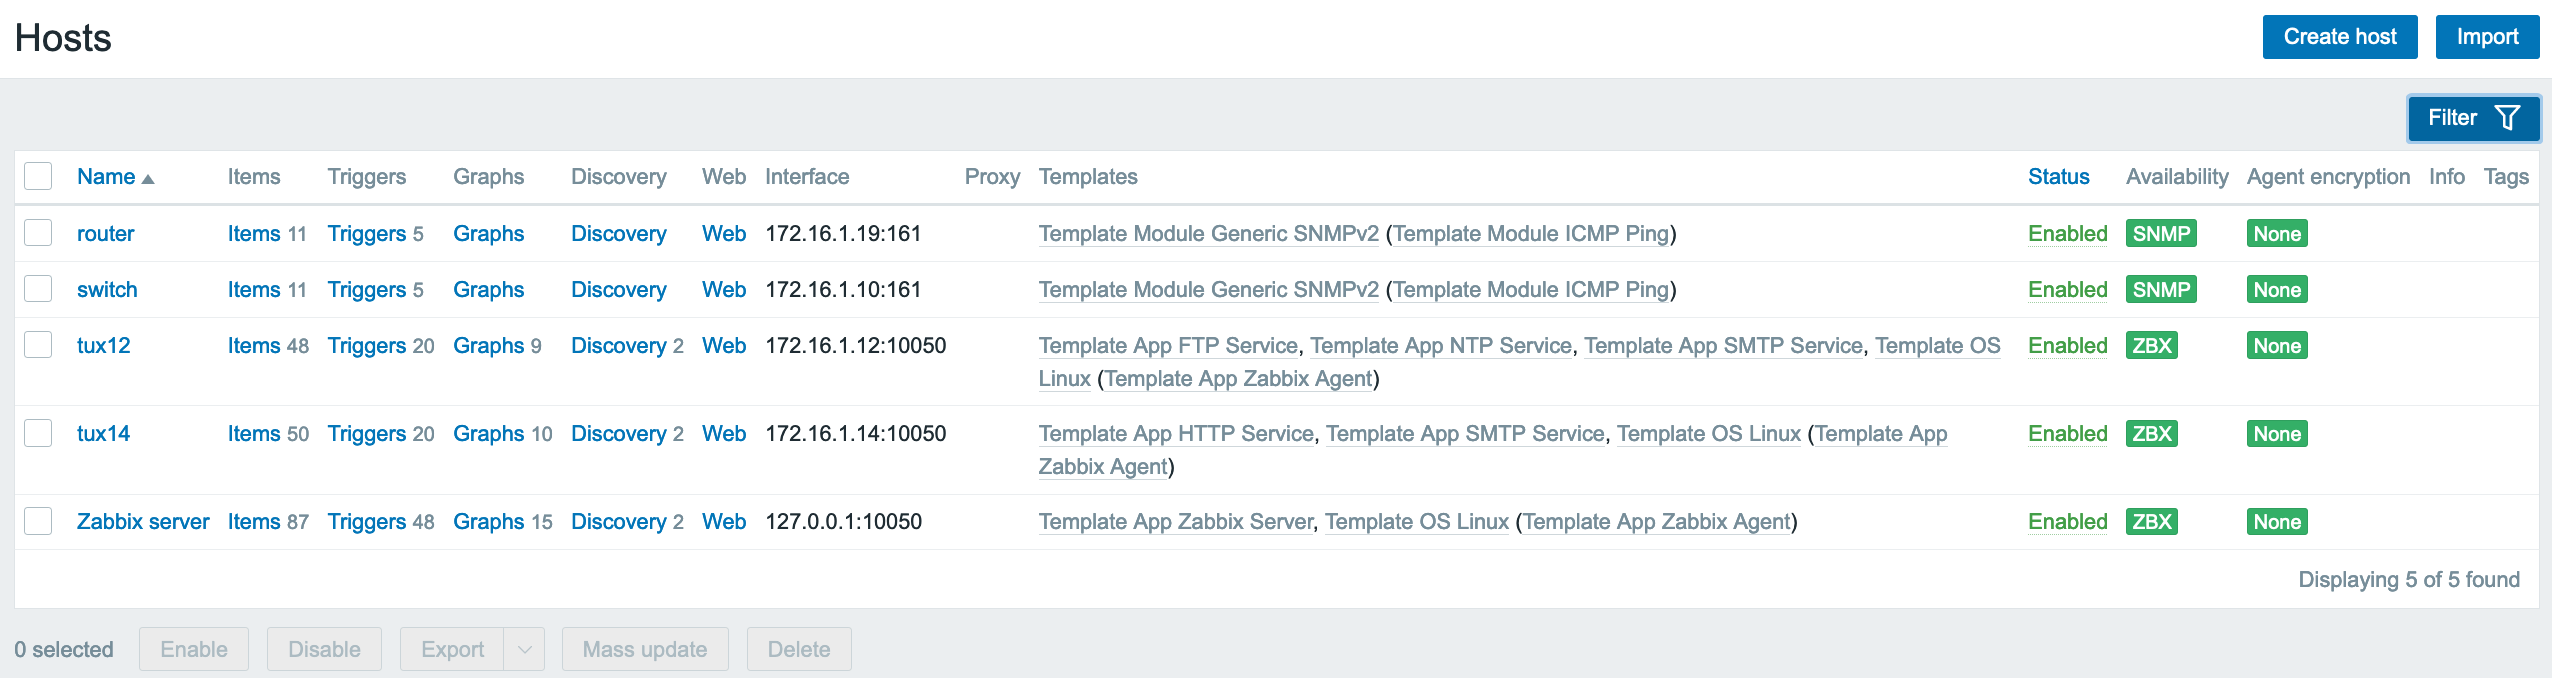
\includegraphics[width=\linewidth]{figs/zabbix/hosts_templates}
    \caption{Templates associados a cada host}
    \label{fig:hosts_templates}
\end{figure}


Como se pode observar, nenhum template associado ao serviço DNS foi adicionado.
De facto, o Zabbix não fornece nenhum template default para esse fim.
Embora seja possível importar templates externos, foi configurado um item e o correspondente trigger manualmente.

\begin{figure}[H]
    \centering
    \begin{subfigure}[b]{0.49\textwidth}
        \centering
        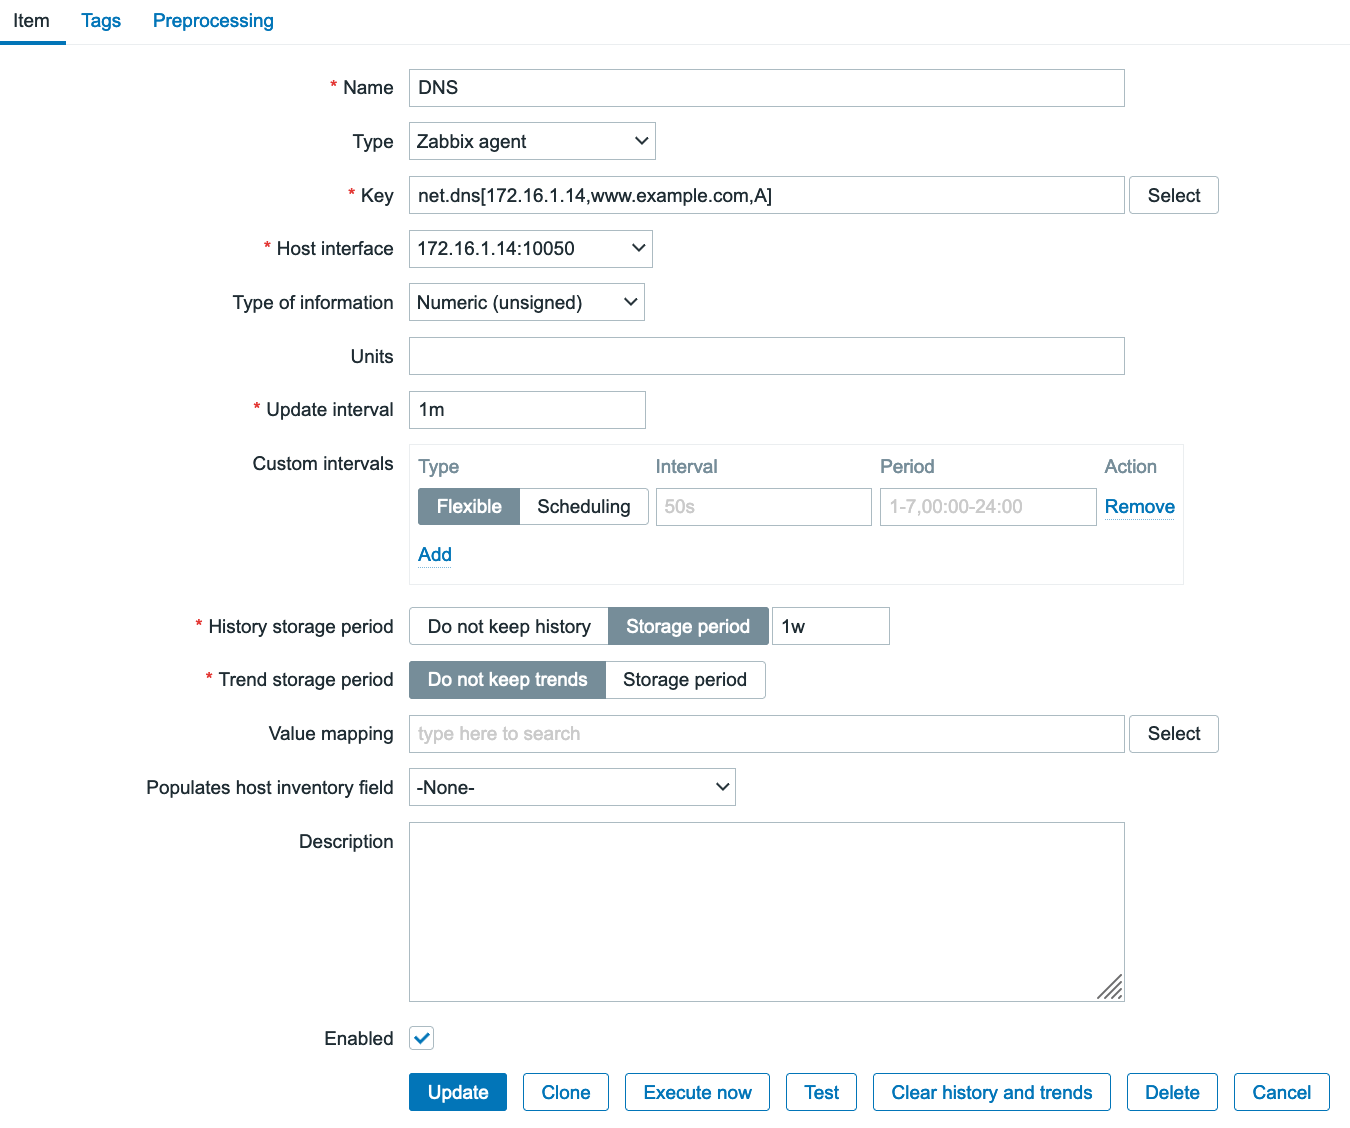
\includegraphics[width=.9\linewidth]{figs/zabbix/dns_item}
        \caption{Item DNS}
        \label{fig:dns_item}
    \end{subfigure}
    \hfill
    \begin{subfigure}[b]{0.49\textwidth}
        \centering
        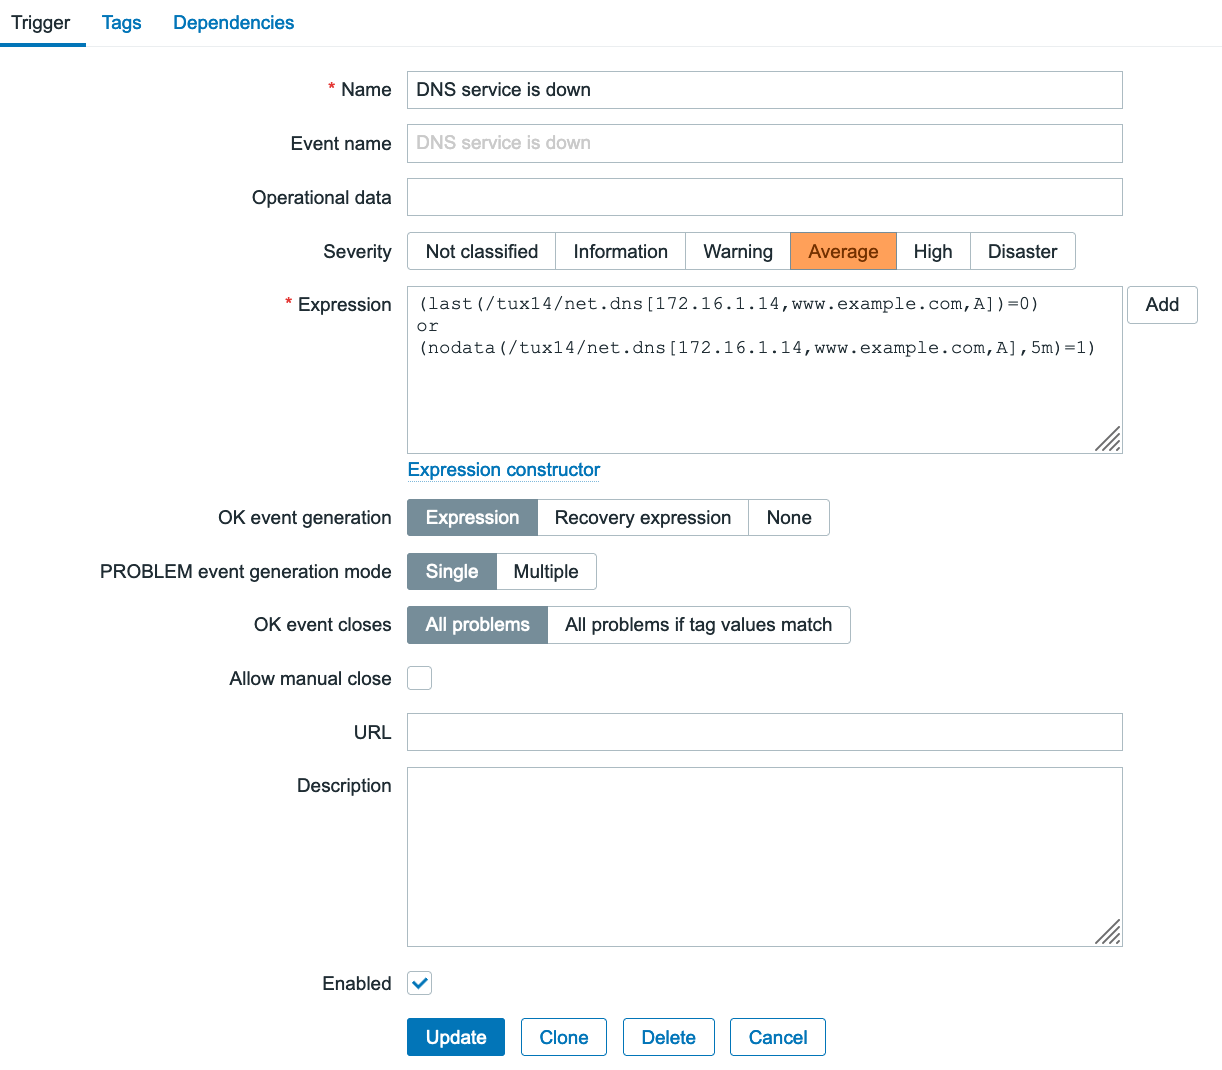
\includegraphics[width=.9\linewidth]{figs/zabbix/dns_trigger}
        \caption{Trigger DNS}
        \label{fig:dns_trigger}
    \end{subfigure}
    \caption{}
\end{figure}

Este teste verifica se a \textit{query} feita ao servidor DNS é respondida. 
Se tal não se verificar, ou se não se obtiver resposta do host de todo, um alerta da gravidade \textit{Average}, igual ao de outros serviços, é criado.

\pagebreak

\section{Resultados}


\begin{figure}[H]
    \centering
    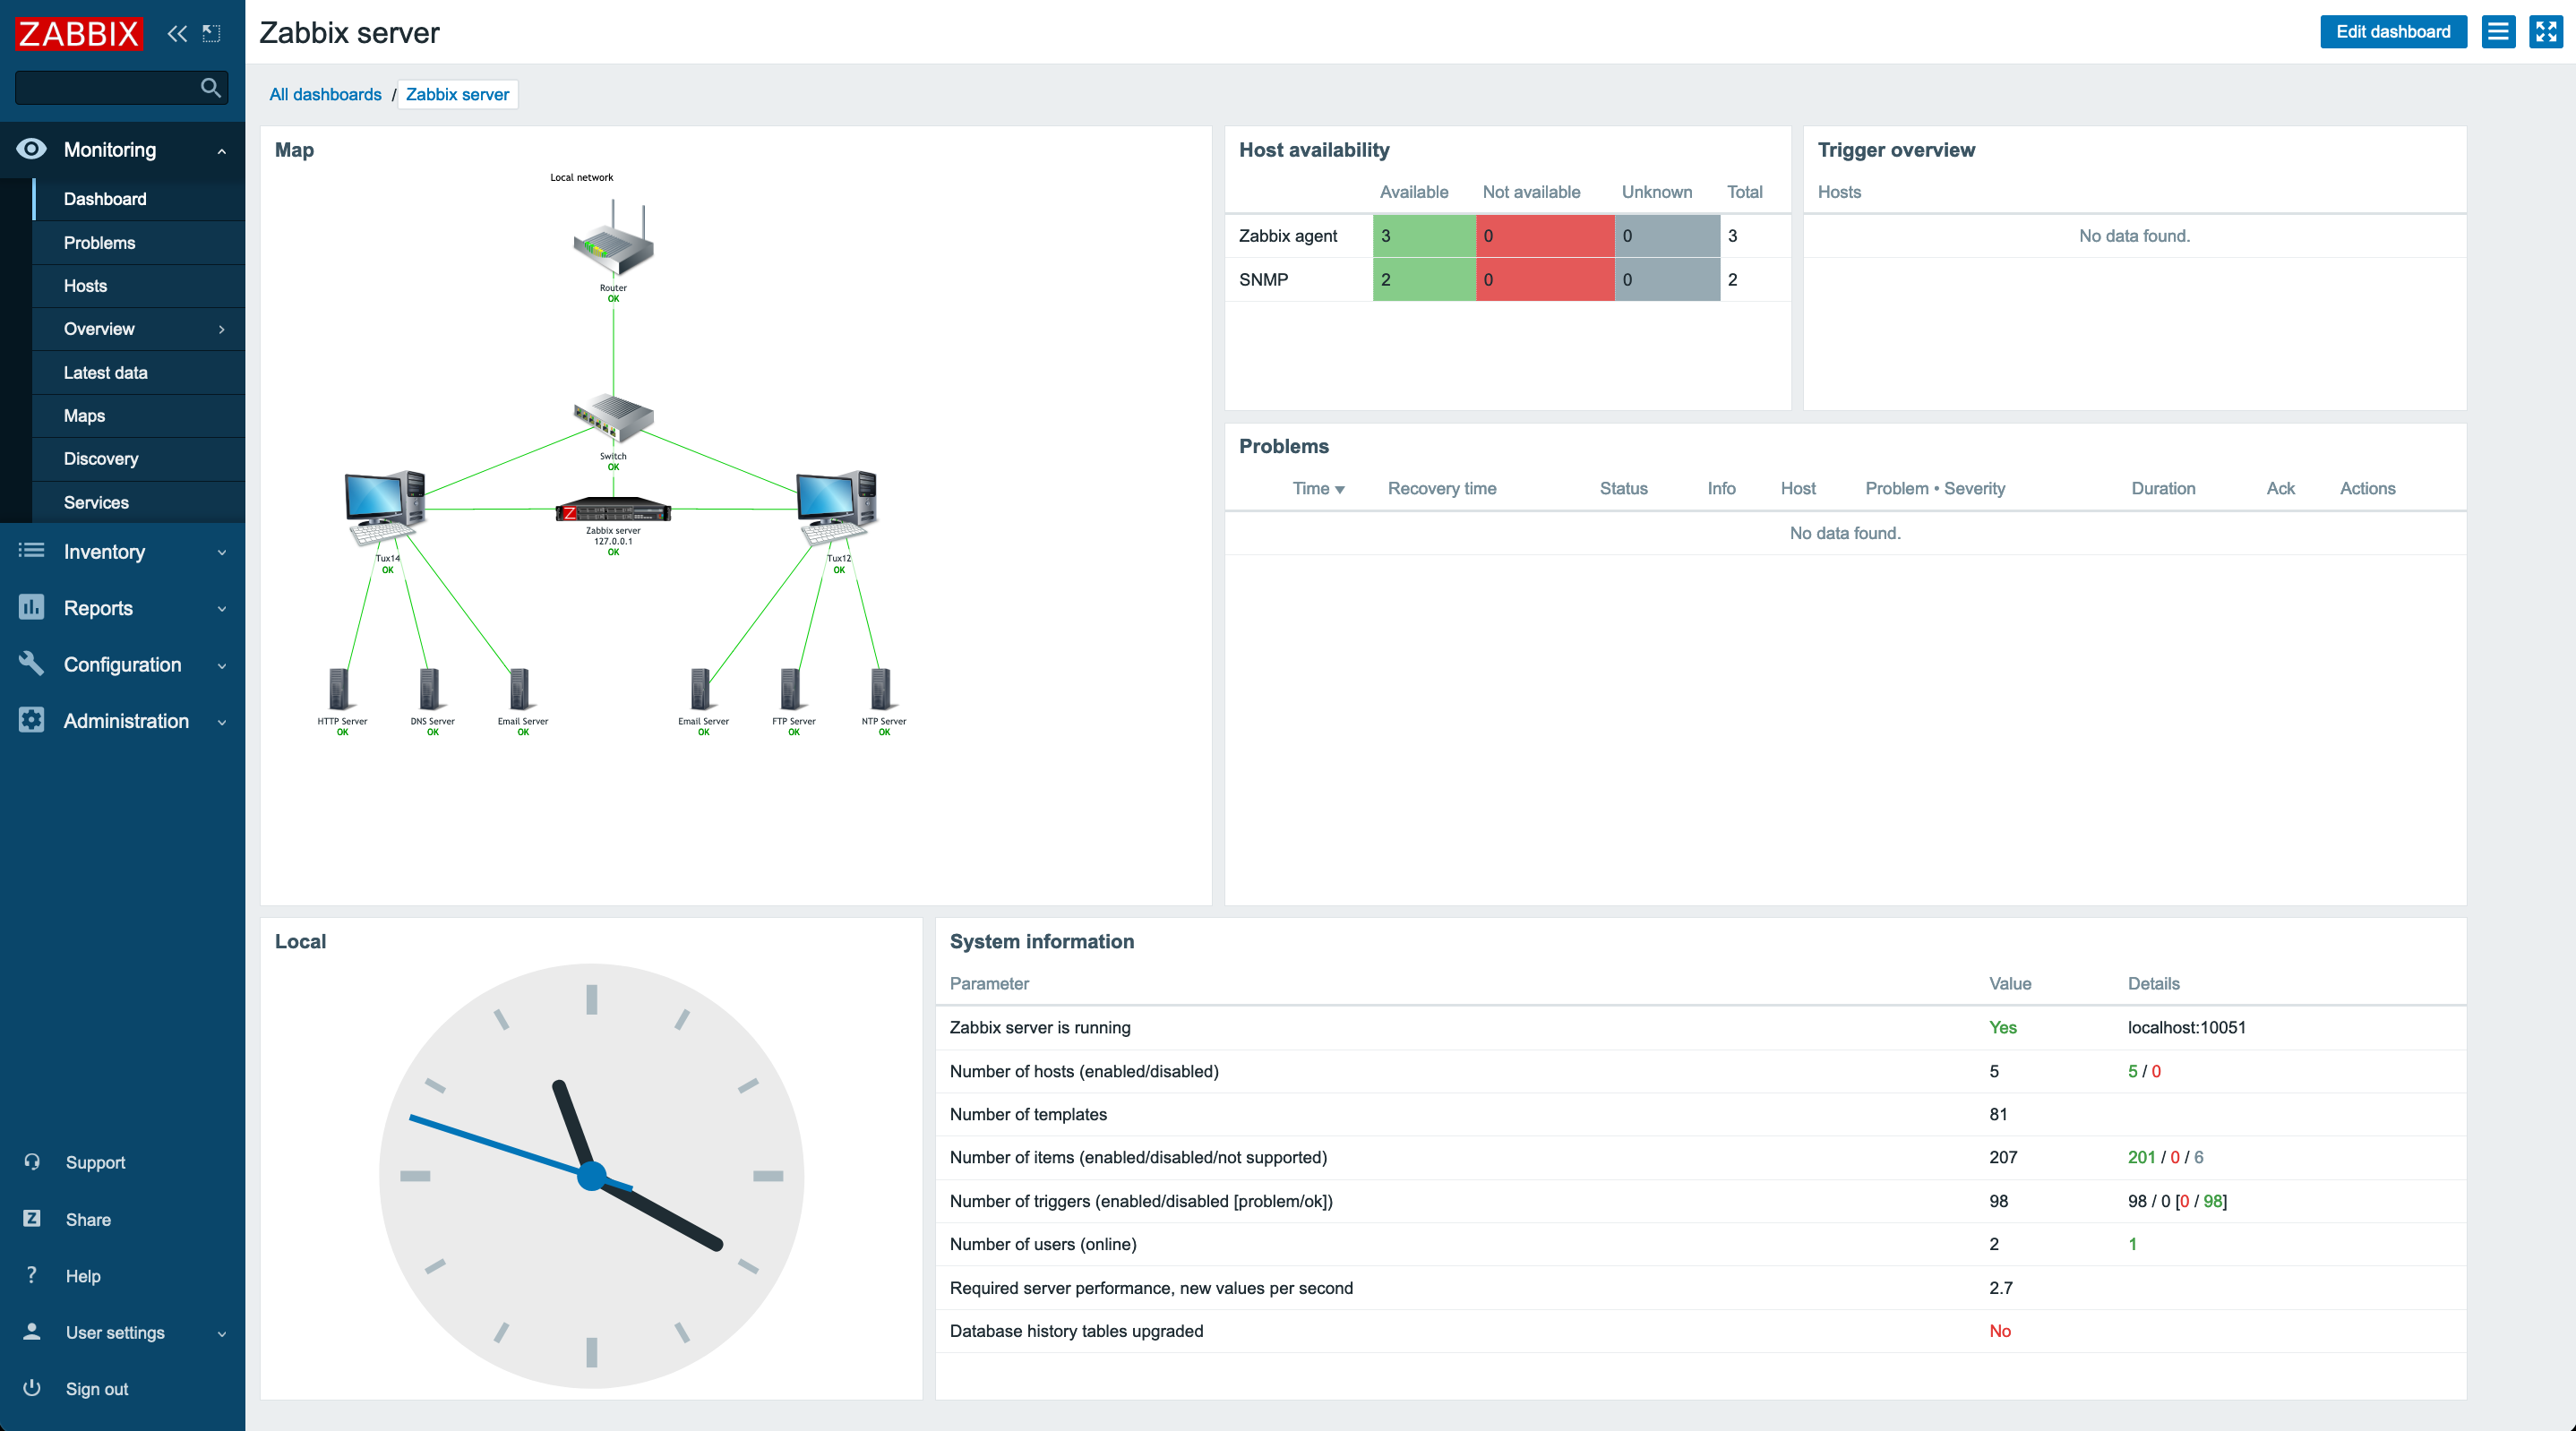
\includegraphics[width=\linewidth]{figs/zabbix/zabbix_dashboard}
    \caption{Dashboard principal}
    \label{fig:zabbix_dashboard}
\end{figure}

Uma das principais vantagens do Zabbix é o seu grau de customização, nomeadamente as \textbf{Dashboards}.
Esta dashboard foi criada por nós, onde a informação mais relevante é apresentada:
\begin{itemize}
    \item Hosts Availability: Quantos hosts então \textit{up/down}.
    \item Trigger Overview: Quais foram os triggers que foram despoletados.
    \item Problems: Quais os problemas do rede.
    \item System Information: Compilação geral da configuração do sistema e status da rede.
    \item Local: Hora local definida no servidor, neste caso \textit{Europe/Lisbon}.
    \item MAP: Interface que permite de uma forma visual verificar o status de serviços e hosts.
    Este mapa foi desenhado por nós para apresentar todos os hosts e os serviços neles alojados.
    É possívelmente a componente mais importante pois apresenta pragmaticamente e de forma simples toda a informação relevante neste trabalho.
\end{itemize}

Existem muitas outras interfaces com compilação de informação do sistema.
É também possível ver a evolução do status de alguns parâmetros graficamente ou o histórico de outputs.

\pagebreak

\section{Teste de falhas}

Os testes de falhas no Nagios e no Zabbix foram executados ao mesmo tempo, pelo que o método é o mesmo:
\begin{center}
    Tux12 \\
    \verb|systemctl stop vsftpd - Falha do servidor FTP| \\
    \verb|systemctl stop postfix - Falha do servidor Email| \\

    \vspace{1cm}
    Tux14 \\
    \verb|systemctl stop bind9 - Falha do servidor DNS| \\
    \verb|systemctl stop apache2 - Falha do servidor HTTP|
\end{center}

Após algum tempo de atualização de informação, o output da interface do Zabbix foi o seguinte:

\begin{figure}[H]
    \centering
    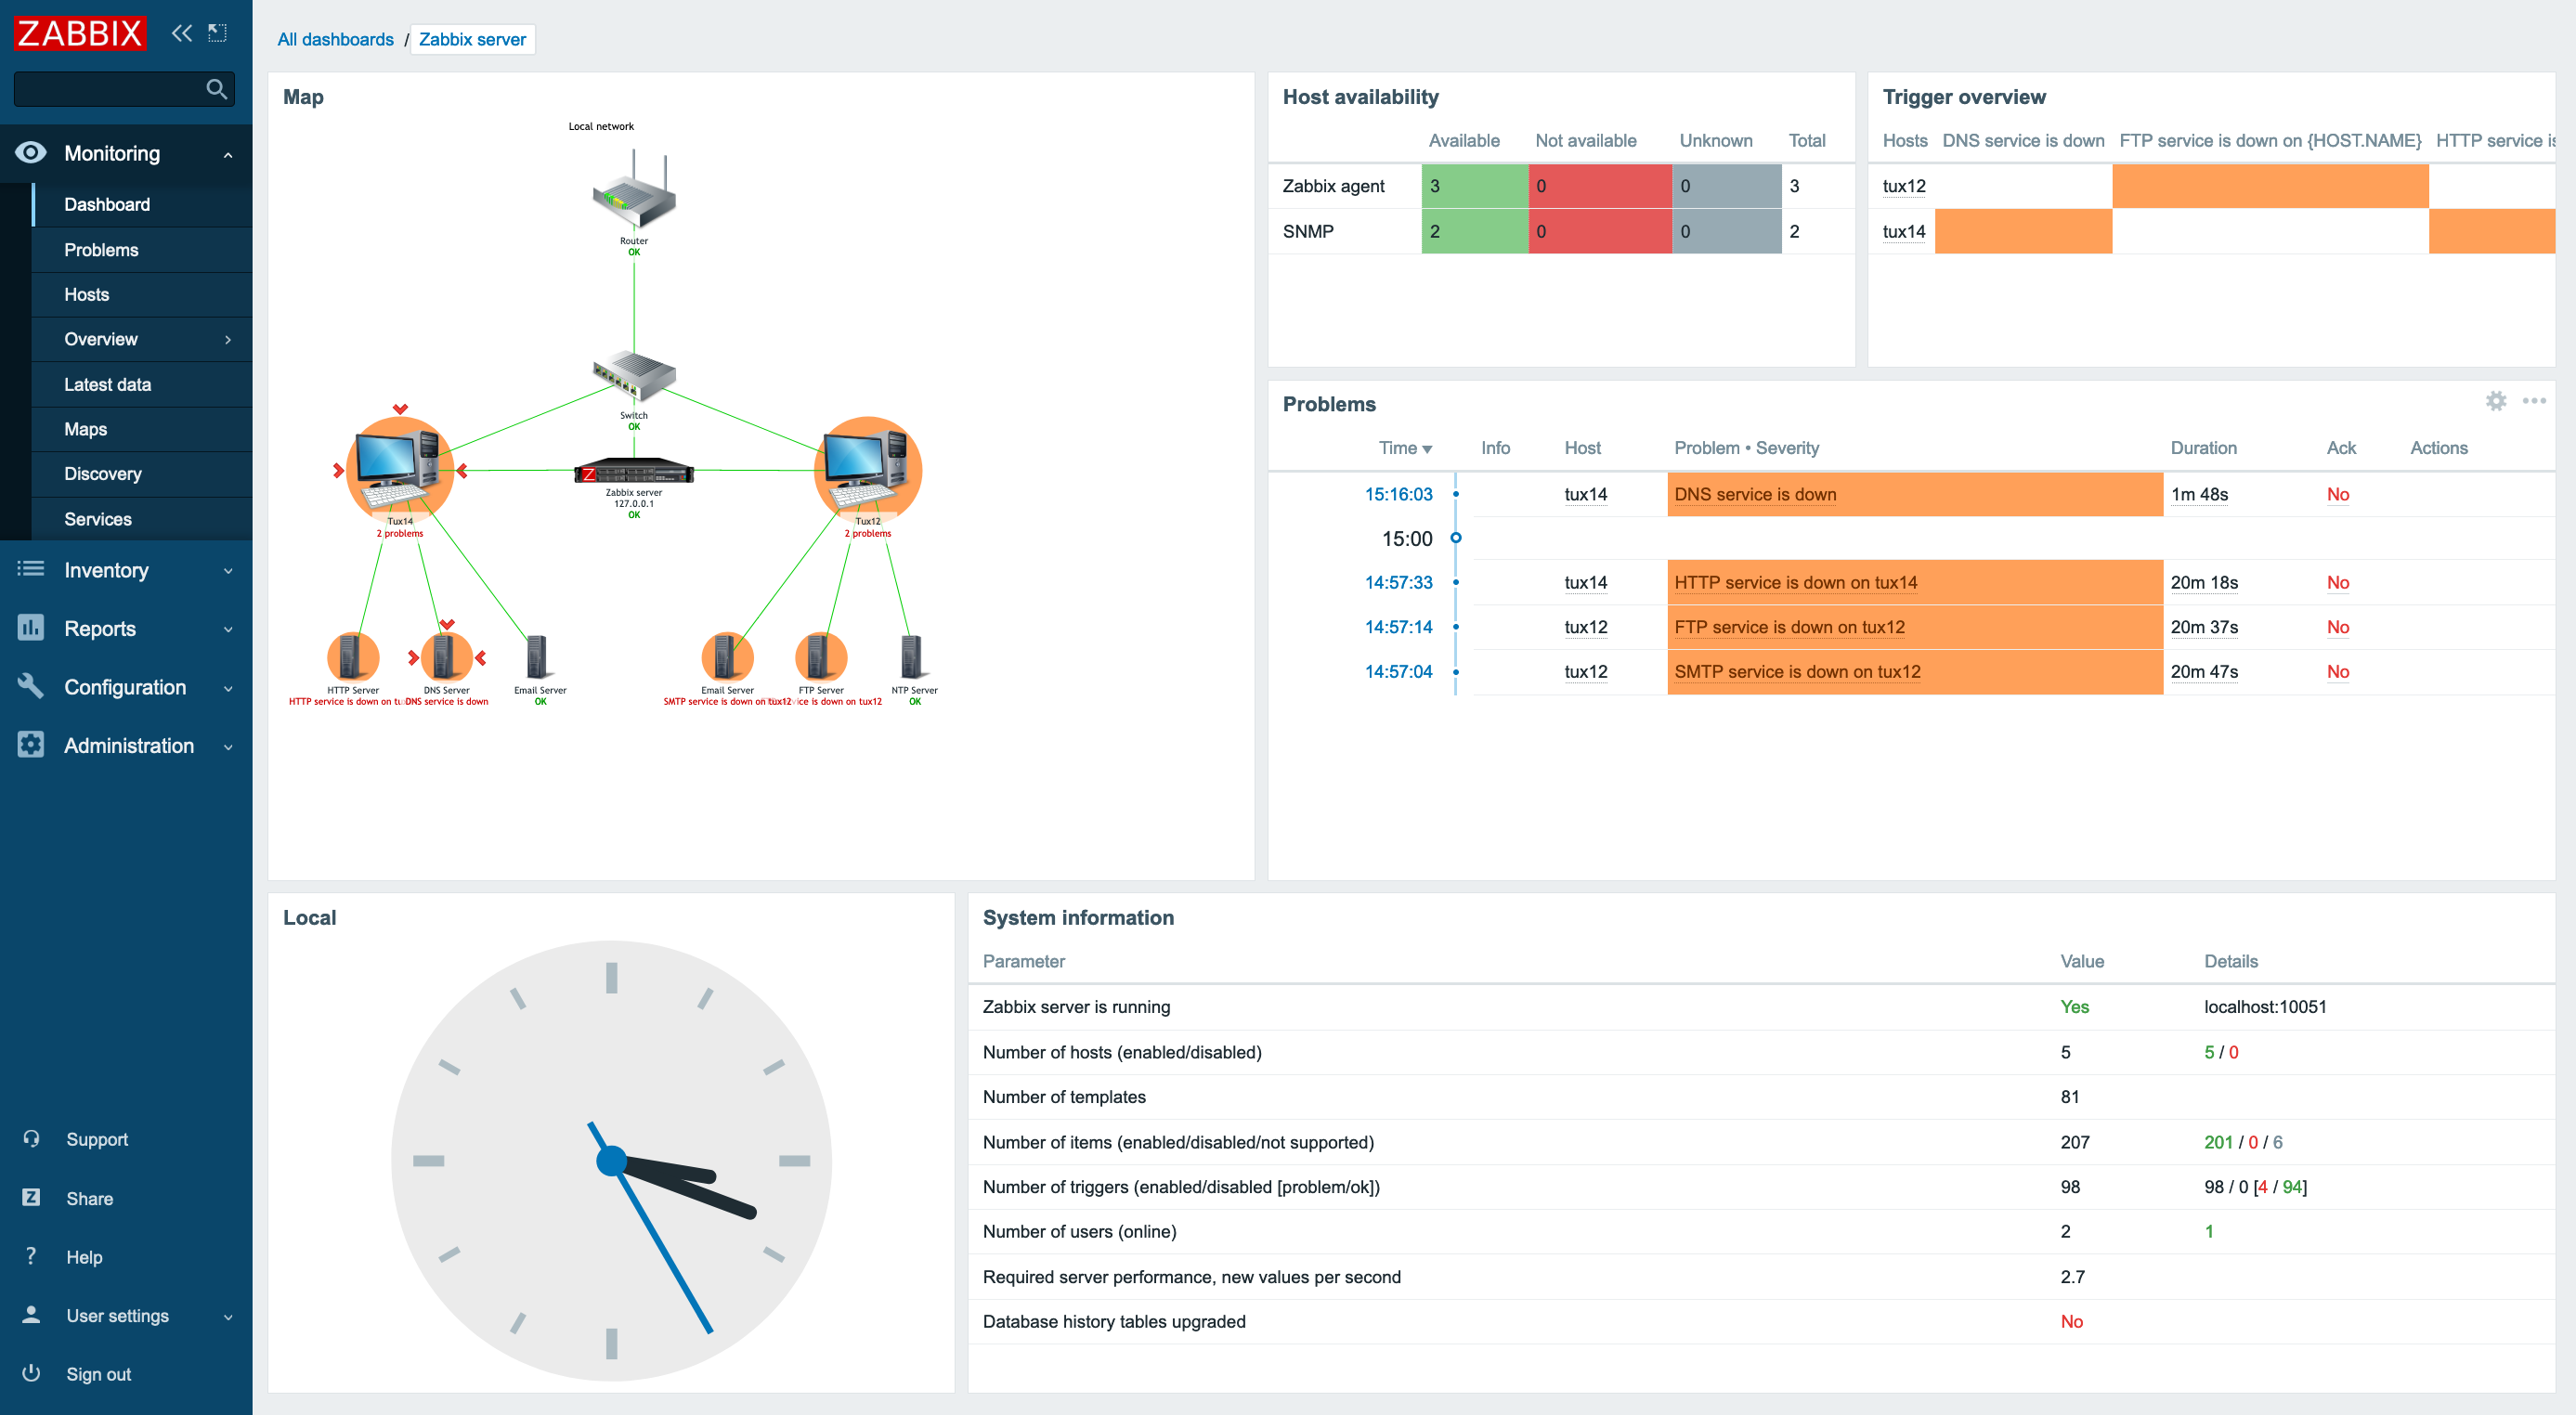
\includegraphics[width=\linewidth]{figs/zabbix/zabbix_errors}
    \caption{Falha de serviços}
    \label{fig:zabbix_errors}
\end{figure}

O Zabbix apresenta na tab \textit{Problems} quais são os problemas encontrados, neste caso os serviços down, assim como o \textit{timestamp} associado ao evento.
É possível também observar quais foram os triggers despoletados, e em que hosts ocorreram.
Por fim, de uma forma mais visual, os hosts onde há problemas são destacados com a cor do problema mais grave, neste caso de severidade \textit{Average} que corresponde ao laranja.

Consequentemente, simulou-se a falha do Tux14, obtendo-se os seguintes resultados:

\begin{figure}[H]
    \centering
    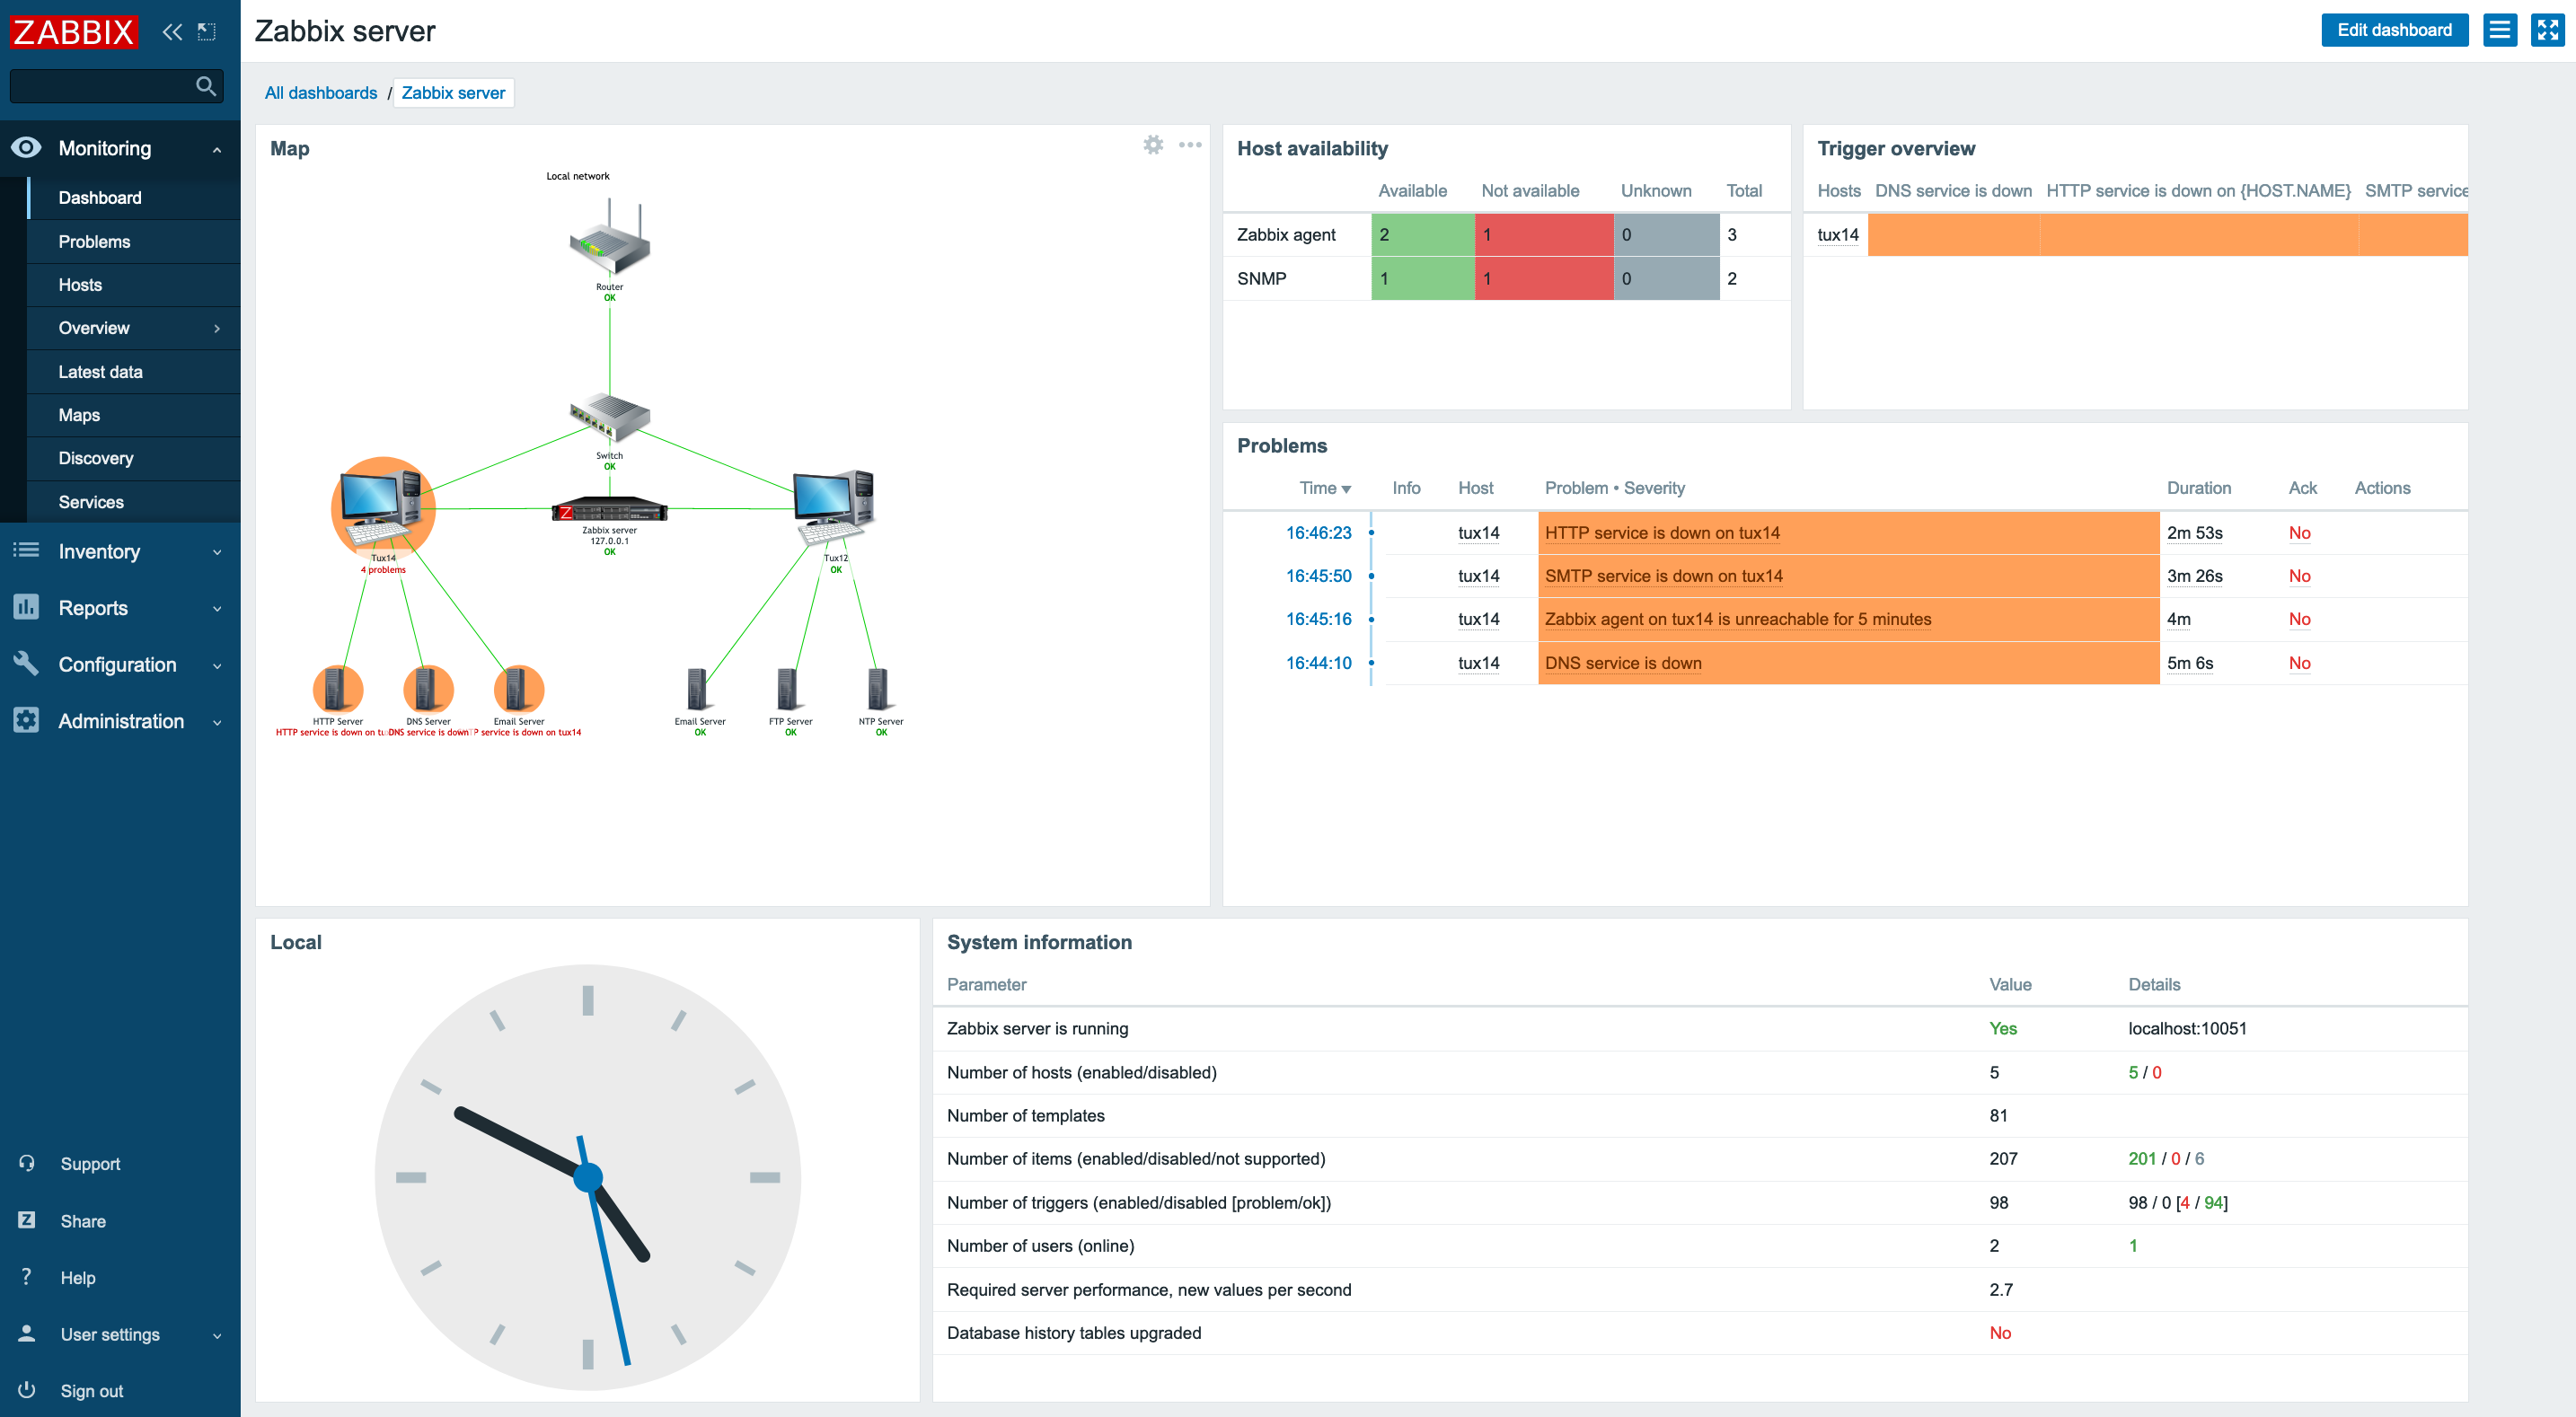
\includegraphics[width=\linewidth]{figs/zabbix/zabbix_tux14_down}
    \caption{Falha do Tux14}
    \label{fig:zabbix_tux14_down}
\end{figure}

É possível observar que o Zabbix indica que se perdeu contacto com o agente no Tux14.
Desse modo, na tab \textit{Host availability}, já se observa que um host está down.
Os serviços alojados no host que falhou também falharam todos, como se pode ver quer no mapa, quer na tab \textit{Problems}.

Sabendo que o host foi desligado às 16:40, o Zabbix demorou 4 minutos a detetar a falhar no sistema, sendo que o estado serviços foi atualizado pouco depois.
É de salientar que a frequência de teste pode ser alterado igualmente na configuração do Zabbix.
\chapter {Outras ferramentas}

\section{Grafana}

\textbf{Grafana} é uma ferramenta \textit{open-source} de monitorização \cite{Grafana}.
Esta ferramenta destaca-se pela sua interface UI muito interativa, apresentando vários gráficos e \textit{gauges}.
Deste modo, é possível criar dashboards muitos customizáveis e dinâmicas.

Ao contrário do Nagios e do Zabbix, este software é desenvolvido com um backend em \textit{Go Lang}, uma linguagem mais recente e \textit{higher-level} que \textit{C Lang}.

Devido a ser uma ferramenta gráfica poderosa, é utilizada em complemento com ferramentas mais específicas mas não tão gráficas como o Zabbix, fornecendo assim informação high-level diretamente ao utilizador.

\begin{figure}[H]
    \centering
    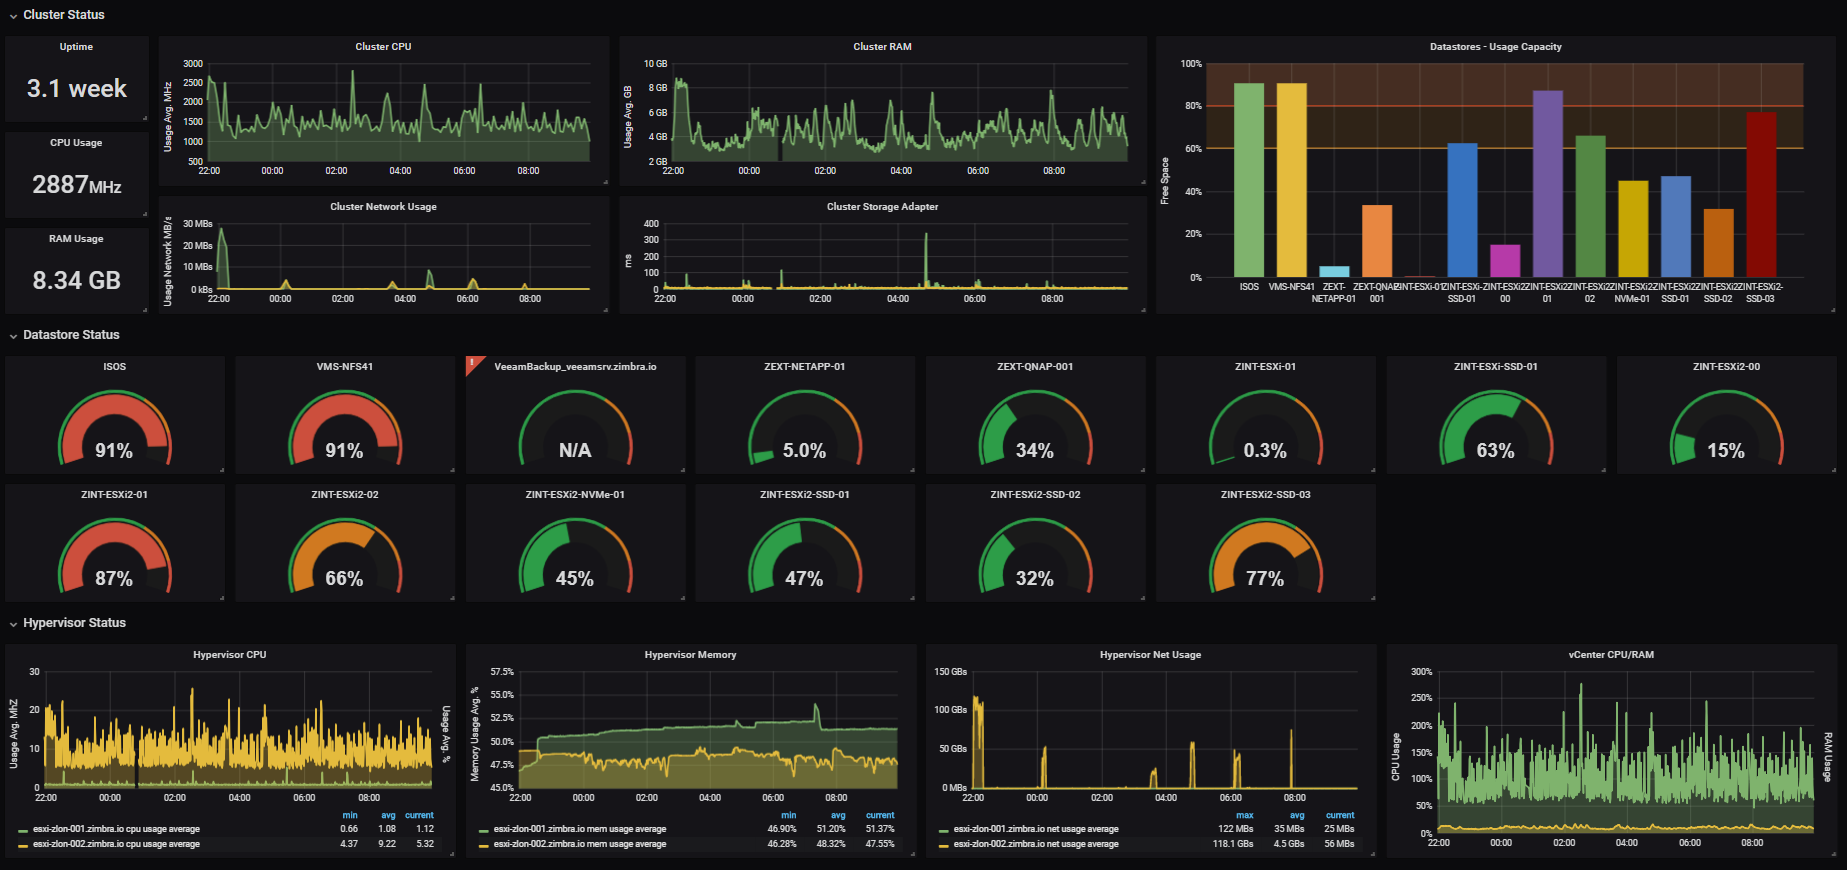
\includegraphics[width=\linewidth]{figs/others/grafana}
    \caption{UI do Grafana}
    \label{fig:grafana}
\end{figure}

\pagebreak

\section{openDCIM}

\textbf{openDCIM} é outra ferramenta de monitorização \textit{open-source} orientada para \textit{data centers} \cite{openDCIM}.
De facto, DCIM significa \textit{Data Center Infrastructure Management}.
É uma ferramenta mais específica, guardando informação relativa ao próprio hardware, sendo possível registar todo o inventário de equipamentos.
É possível também realizar testes da própria infraestrutura de rede, simulando por exemplo um corte de energia e analisando os serviços afetados.

No entanto, a UI dessa desta ferramenta é muito mais simples e mais antiga, não sendo possível ter uma interface gráfica customizável como por exemplo com o Grafana.
Disponibiliza também menos ferramentas de análise de serviços do que as outras opções.

\begin{figure}[H]
    \centering
    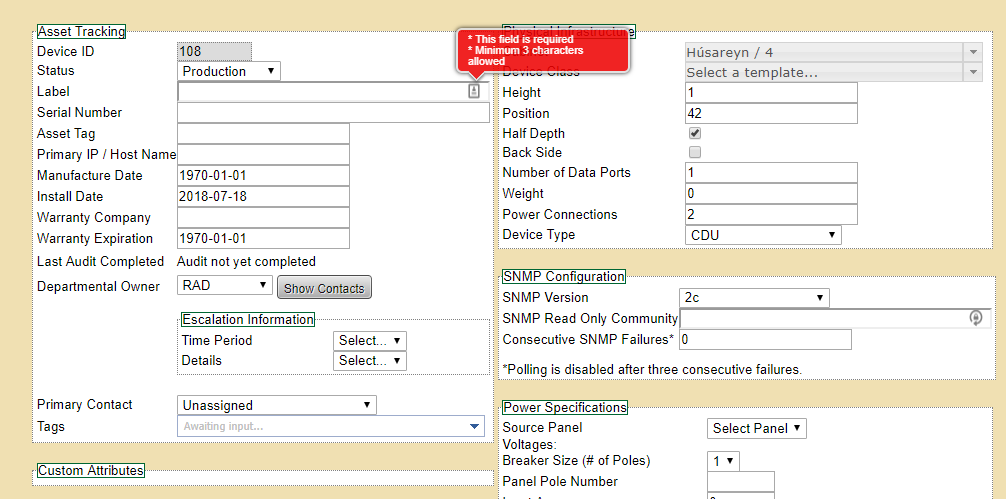
\includegraphics[width=\linewidth]{figs/others/opendcim}
    \caption{UI do openDCIM}
    \label{fig:opendcim}
\end{figure}



\chapter{Análise comparativa}

Após os testes dos diferentes serviços, é possível fazer uma comparação direta e determinar qual a melhor ferramenta em cada contexto.


\section*{Interface gráfica}

O \textbf{Grafana} é a ferramenta que proporciona a melhor experiência gráfica ao utilizador.
Como uma UI muito focada em gráficos temporais e \textit{gauges}, é bastante fácil e intuitivo rapidamente analisar o estado do sistema.

O \textbf{Zabbix} no entanto também tem uma excelente interface, principalmente com a funcionalidade de construção de mapas que permitem esquematizar a rede e o seu estado.
Além disso, fornece mais informação, principalmente low-level do que o \textbf{Nagios}.

\section*{Configuração}
Neste ponto apenas é possível comparar a duas ferramentas usadas.
A configuração no \textbf{Zabbix} é feita na sua interface Web, pelo que desse modo é muito mais intuitivo e simples modificar e personalizar a ferramenta.
Apesar do \textbf{Nagios} também ser muito configurável, é preciso modificar os ficheiros .conf diretamente no sistema, o que torna a experiência mais complexa e menos intuitiva.

Outro fator prende-se com abordagem dos templates, que permite anexar rapidamente um conjunto de teste relevantes naquele contexto, por exemplo de um serviço HTTP ou FTP.
O Nagios por outro lado, obriga a manualmente se configurar cada teste individualmente para cada host, sendo portanto um processo mais moroso.

\section*{Plugins vs Items/Triggers}
Apesar da configuração do \textbf{Nagios} ser mais complexa, os plugins são mais configuráveis do que os items/triggers do \textbf{Zabbix}.

Quando se define um plugin, mais parâmetros podem ser definidos do que num item.
O seu output pode também ser analisado mais precisamente, com intervalos de gravidade, por exemplo, de delay grave ou muito grave.

Além disso, é possível importar facilmente novos plugins como foi feito para o SNMP, enquanto que os items do Zabbix são predefinidos no próprio sistema.

\section*{Outras funcionalidades}

Ambos as ferramentas apresentam a funcionalidade de \textbf{Autodiscovery}.
Esta funcionalidade permite a descoberta de novos hosts que entraram na rede local.
No entanto, apenas o Nagios XI (pago) tem esta funcionalidade por predefinição, pelo que desse modo é mais fácil configurar no Zabbix.

A nível de \textbf{protocolos de comunicação suportados}, distingui-se o facto do \textbf{Grafana} suportar mais tipos de bases de dados, nomeadamente em cloud como é o caso da AWS e Azure.
Isto é sem dúvida um fator importante, principalmente para sistemas muito grandes onde é preciso grande capacidade de armazenamento.

Por fim, é possível, quer no Nagios, quer no Zabbix, \textbf{agendar manutenção}, isto é, \textit{downtime} aceitável, aparecendo essa informação disponível na plataforma.

\section{Conclusão}
\begin{frame}{Conclusão}{}
    \begin{itemize}
        \item Fundamentos teóricos da Tonalidade
        \item Algoritmos de deteção
        \begin{itemize}
            \item Krumhansl-Schmukler
        \end{itemize}
        \item Key Profiles
        \begin{itemize}
            \item Krumhansl
            \item Temperley
            \item etc.
        \end{itemize}
        \item Implementação em Python
        \begin{itemize}
            \item Music21
        \end{itemize}
        \item Análise de precisão
        \begin{itemize}
            \item Melhorias no algoritmo
        \end{itemize}
    \end{itemize}
\end{frame}





%Glossary
\clearpage
\printnoidxglossaries

\printbibliography[heading=bibintoc,title={Bibliografia}]
\label{bib:mybiblio}

\clearpage

\end{document}
\grid
\grid
